\subsection{Simulazioni con campo magnetico $h\,=\,0.02$}

La prima fase della simulazione del modello di Ising 1D è incentrata sulla determinazione dei parametri ottimali per ottenere 
dei valori d'aspettazione statisticamente rilevanti, in modo tale da poter effettuare il confronto con il valor vero noto in letteratura. In 
questa fase preliminare ho lavorato con le seguenti quattro lunghezze del modello di Ising 1D e le seguenti quattro temperature 

\begin{equation}
    l\,\in\,\left\{1000,\,3000,\,6000,\,10000\right\}
    \label{eq: dim_sim_Ising1D}
\end{equation}

\begin{equation}
    T\,\in\,\left\{0.5,\,1.0,\,1.5,\,2.0\right\}
    \label{eq: temp_sim_Ising1D}
\end{equation}

Per ognuna di queste coppie dimensione-temperatura ho considerato quattro seed differenti del generatore di numeri casuali in modo da 
poter analizzare il comportamento del sistema lungo differenti traiettorie nello spazio delle fasi. 



\subsubsection{Termalizzazione}

La lunghezza della fase di termalizzazione dipende fortemente dal valore della temperatura a cui viene svolta la simulazione, come è 
possibile osservare nelle seguenti Figure in cui sono riportati i risultati ottenuti raggruppati per lunghezza della catena di spin. 
La durata maggiore della termalizzazione si ha per la temperatura inferiore, ossia $T\,=\,0.5$, poichè per giungere ad una configurazione 
ordinata (come evidente dal valore della magnetizzazione tendente ad uno) è necessario un tempo computazionale maggiore legato alla 
necessità di orientare tutti gli spin in modo concorde.

\newpage

\vspace*{\fill}

\begin{figure}[htbp]
    \centering
    \begin{minipage}{0.45\textwidth}  
      \centering
      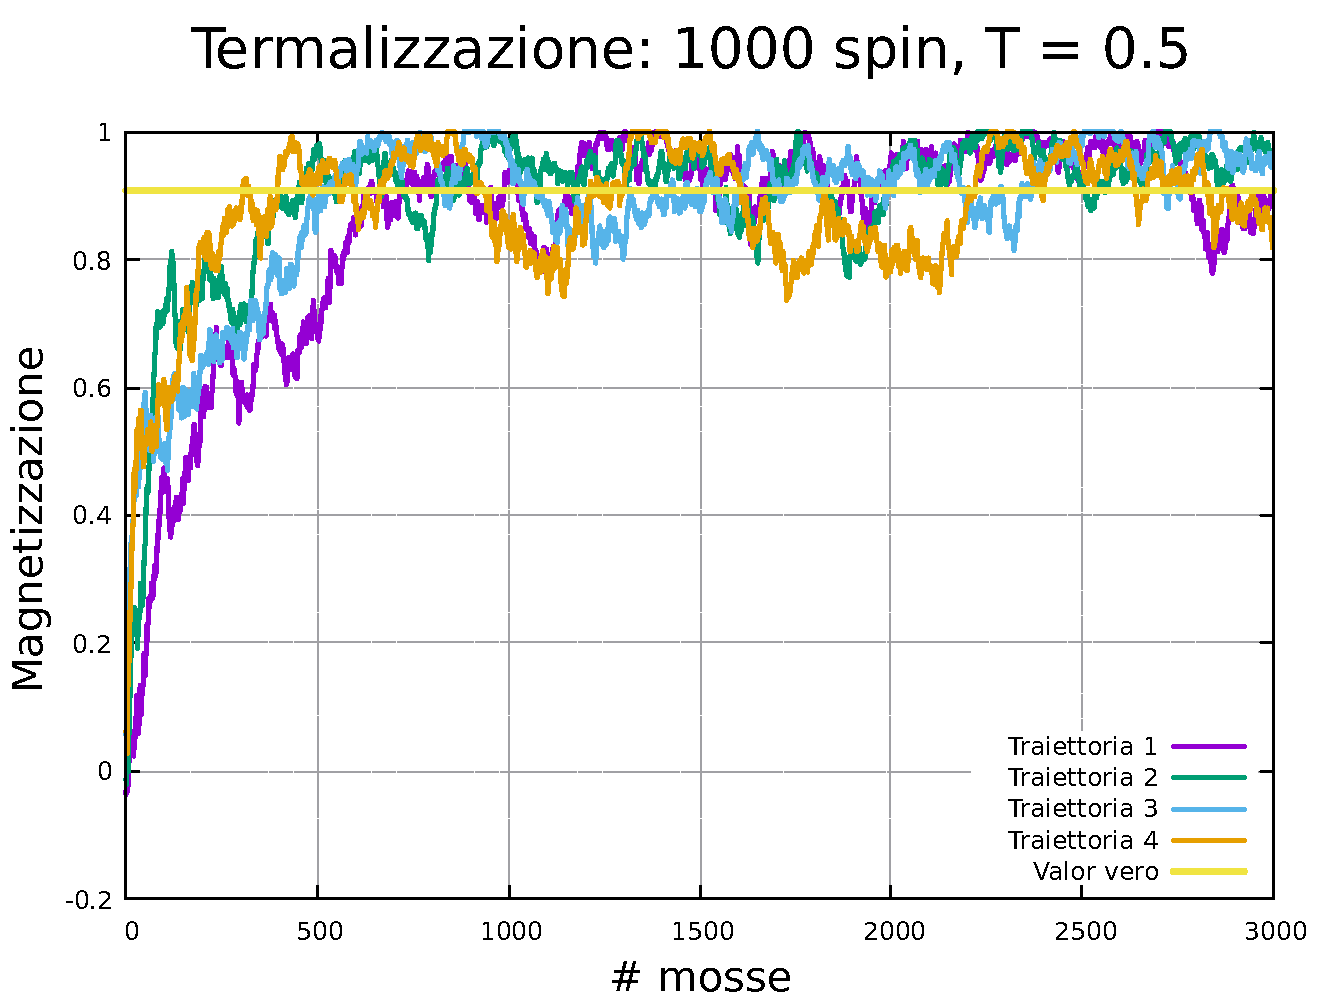
\includegraphics[page=1, width=\textwidth]{Immagini/simIsing1D/magn0.02/term/term_1000_0.5.pdf}
      \caption{$T\,=\,0.5$}
    \end{minipage}\hfill
    \begin{minipage}{0.45\textwidth}  
      \centering
      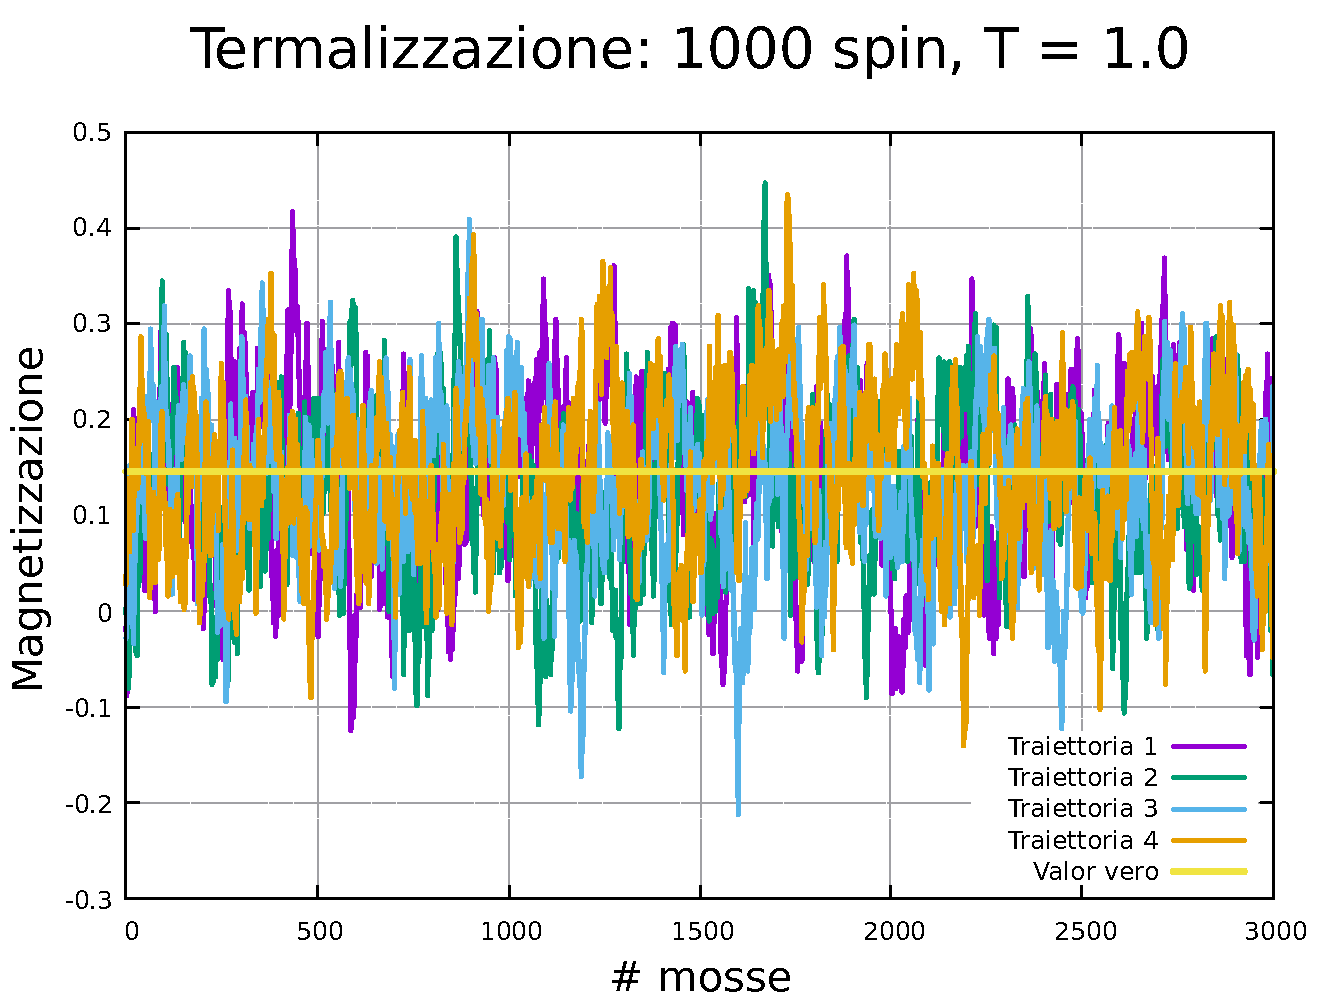
\includegraphics[page=1, width=\textwidth]{Immagini/simIsing1D/magn0.02/term/term_1000_1.0.pdf}
      \caption{$T\,=\,1.0$}
    \end{minipage}
    \vskip\baselineskip 
  
    \begin{minipage}{0.45\textwidth}  
      \centering
      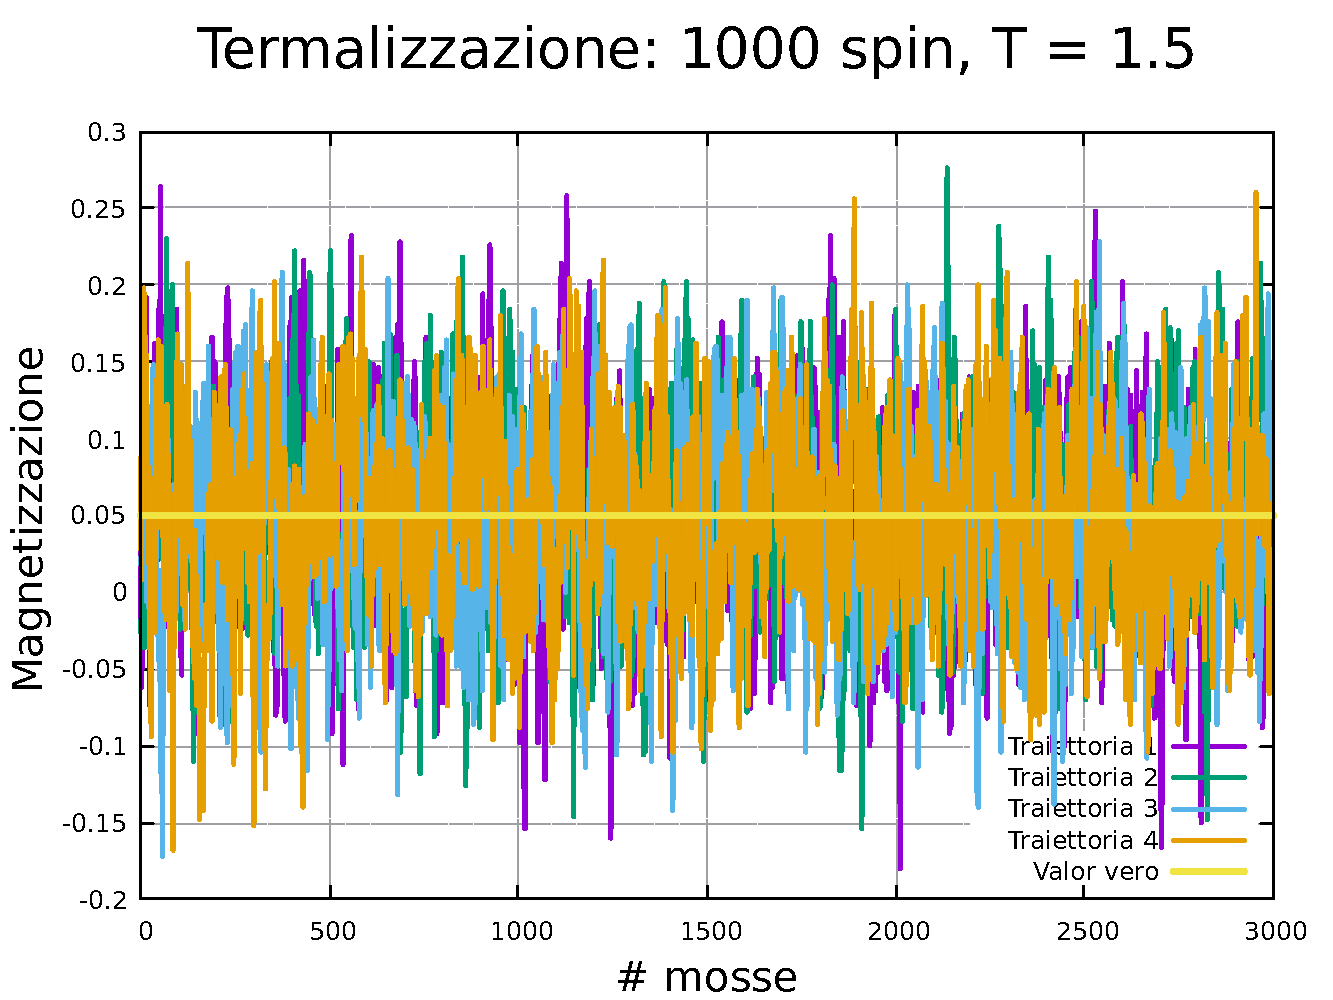
\includegraphics[page=1, width=\textwidth]{Immagini/simIsing1D/magn0.02/term/term_1000_1.5.pdf}
      \caption{$T\,=\,1.5$}
    \end{minipage}\hfill
    \begin{minipage}{0.45\textwidth}  
      \centering
      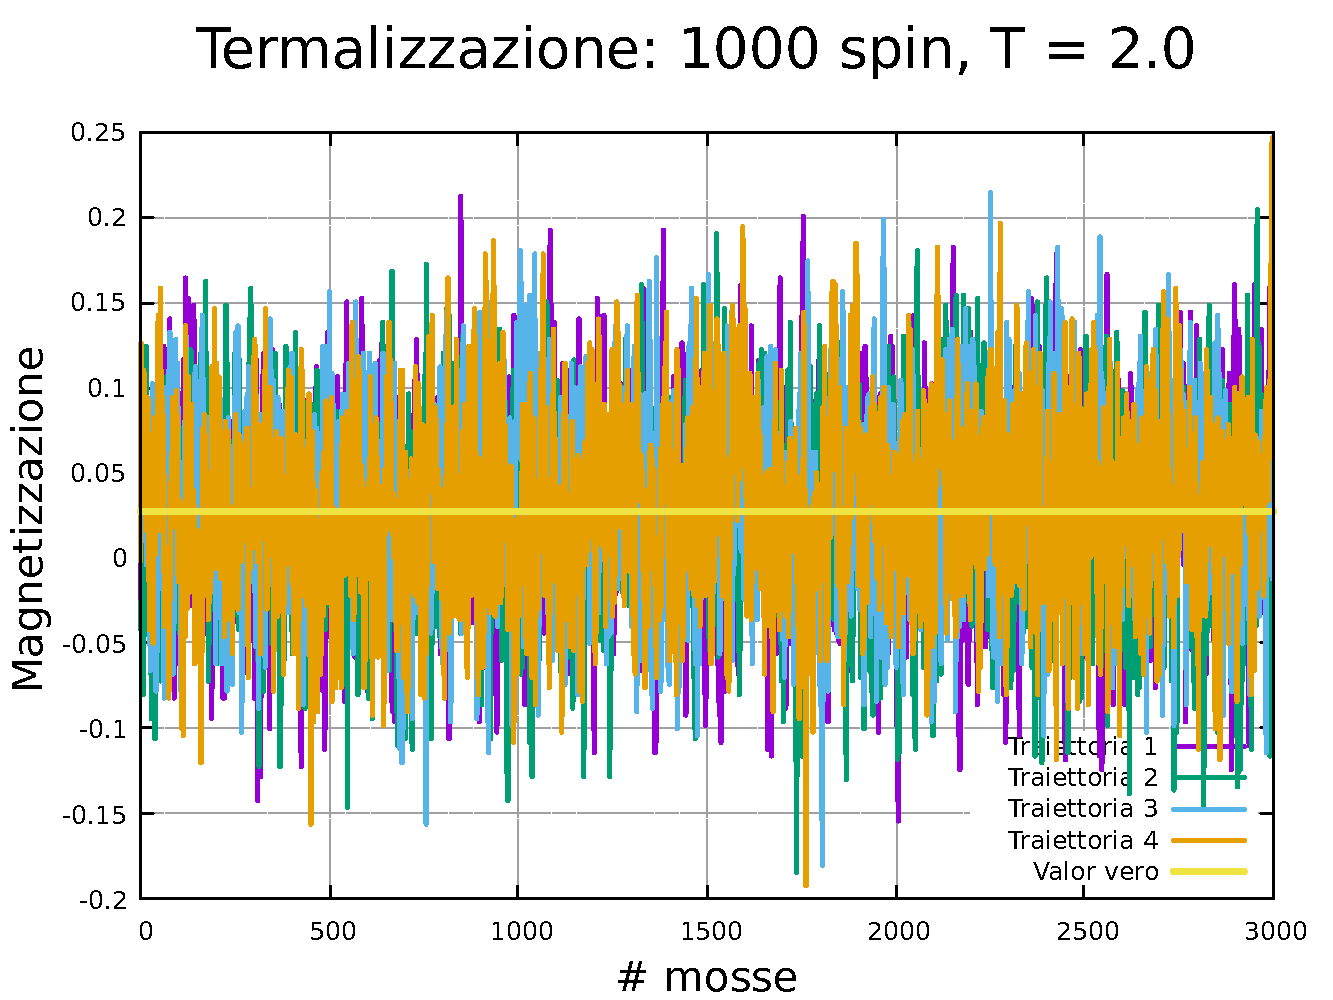
\includegraphics[page=1, width=\textwidth]{Immagini/simIsing1D/magn0.02/term/term_1000_2.0.pdf}
      \caption{$T\,=\,2.0$}
    \end{minipage}
    \caption{Studio della termalizzazione di un modello di Ising 1D costituito da 1000 spin.}
\end{figure}

\vspace*{\fill}

\newpage

\vspace*{\fill}

\begin{figure}[htbp]
    \centering
    \begin{minipage}{0.45\textwidth}  
      \centering
      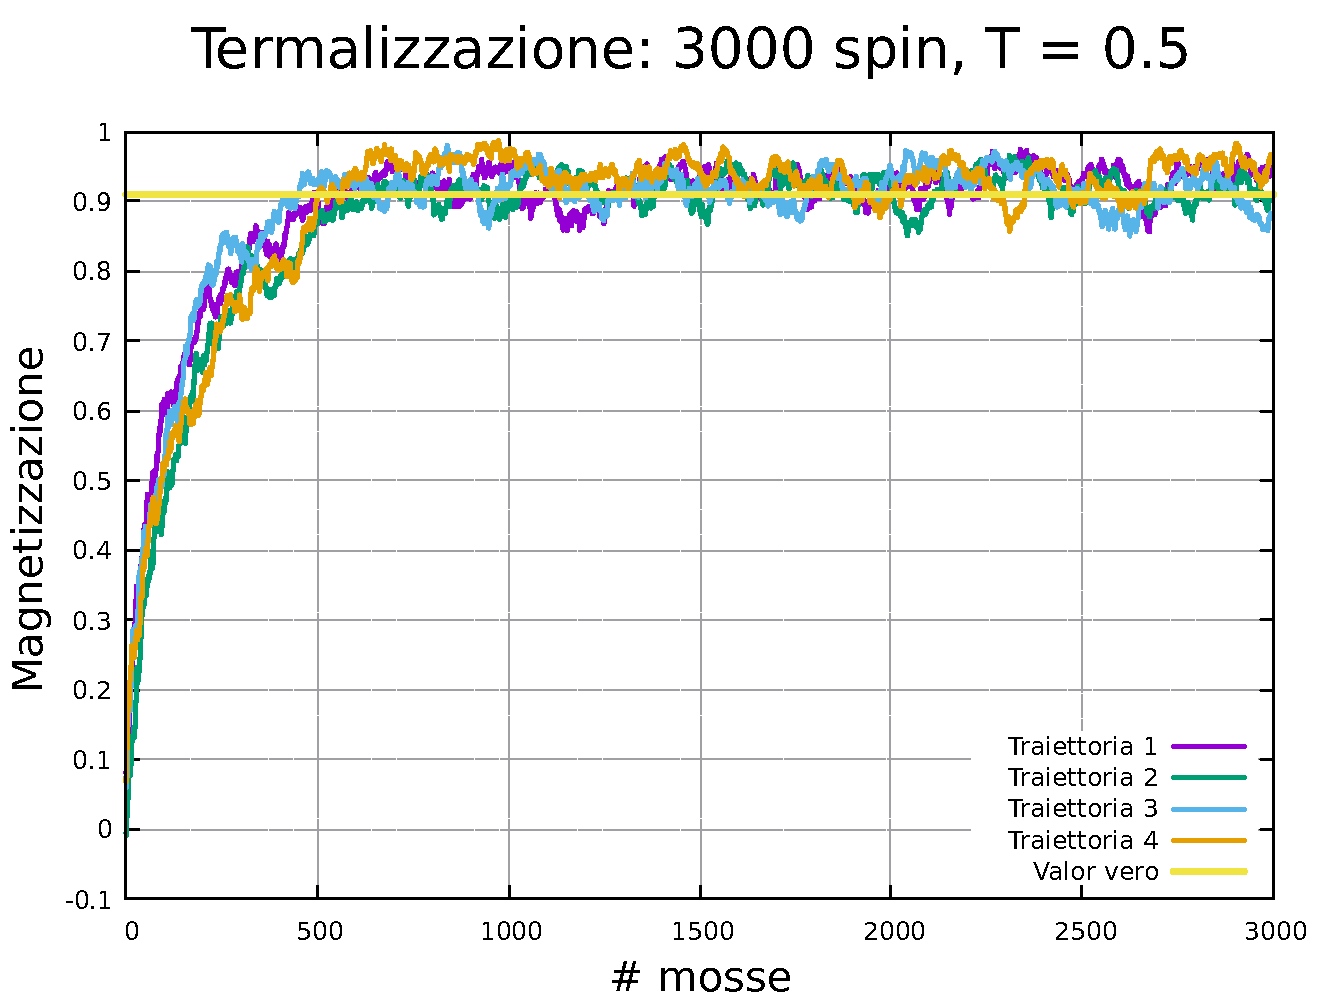
\includegraphics[page=1, width=\textwidth]{Immagini/simIsing1D/magn0.02/term/term_3000_0.5.pdf}
      \caption{$T\,=\,0.5$}
    \end{minipage}\hfill
    \begin{minipage}{0.45\textwidth}  
      \centering
      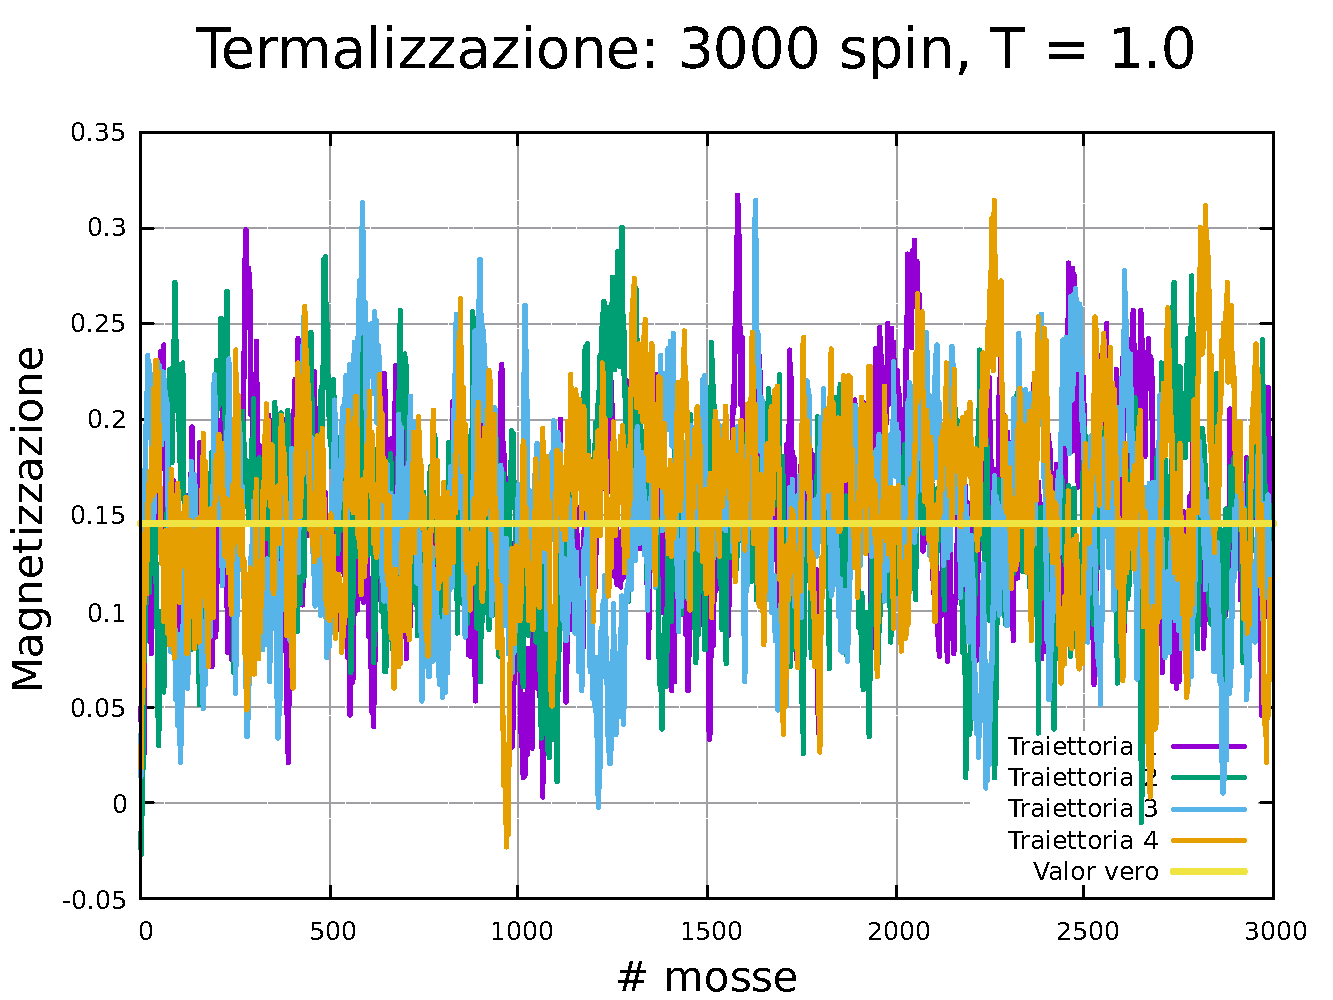
\includegraphics[page=1, width=\textwidth]{Immagini/simIsing1D/magn0.02/term/term_3000_1.0.pdf}
      \caption{$T\,=\,1.0$}
    \end{minipage}
    \vskip\baselineskip 
  
    \begin{minipage}{0.45\textwidth}  
      \centering
      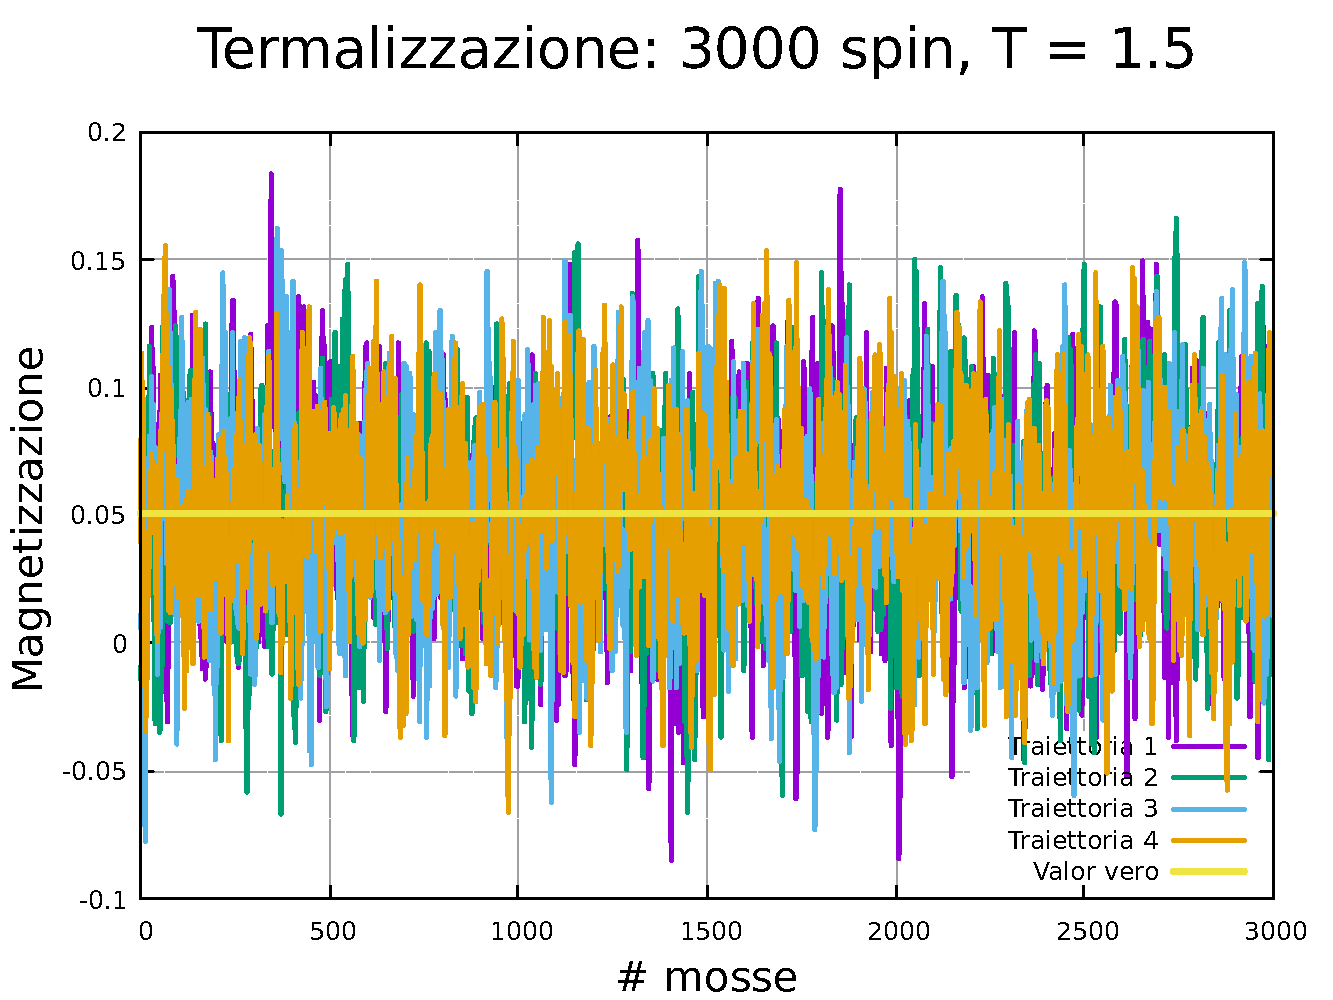
\includegraphics[page=1, width=\textwidth]{Immagini/simIsing1D/magn0.02/term/term_3000_1.5.pdf}
      \caption{$T\,=\,1.5$}
    \end{minipage}\hfill
    \begin{minipage}{0.45\textwidth}  
      \centering
      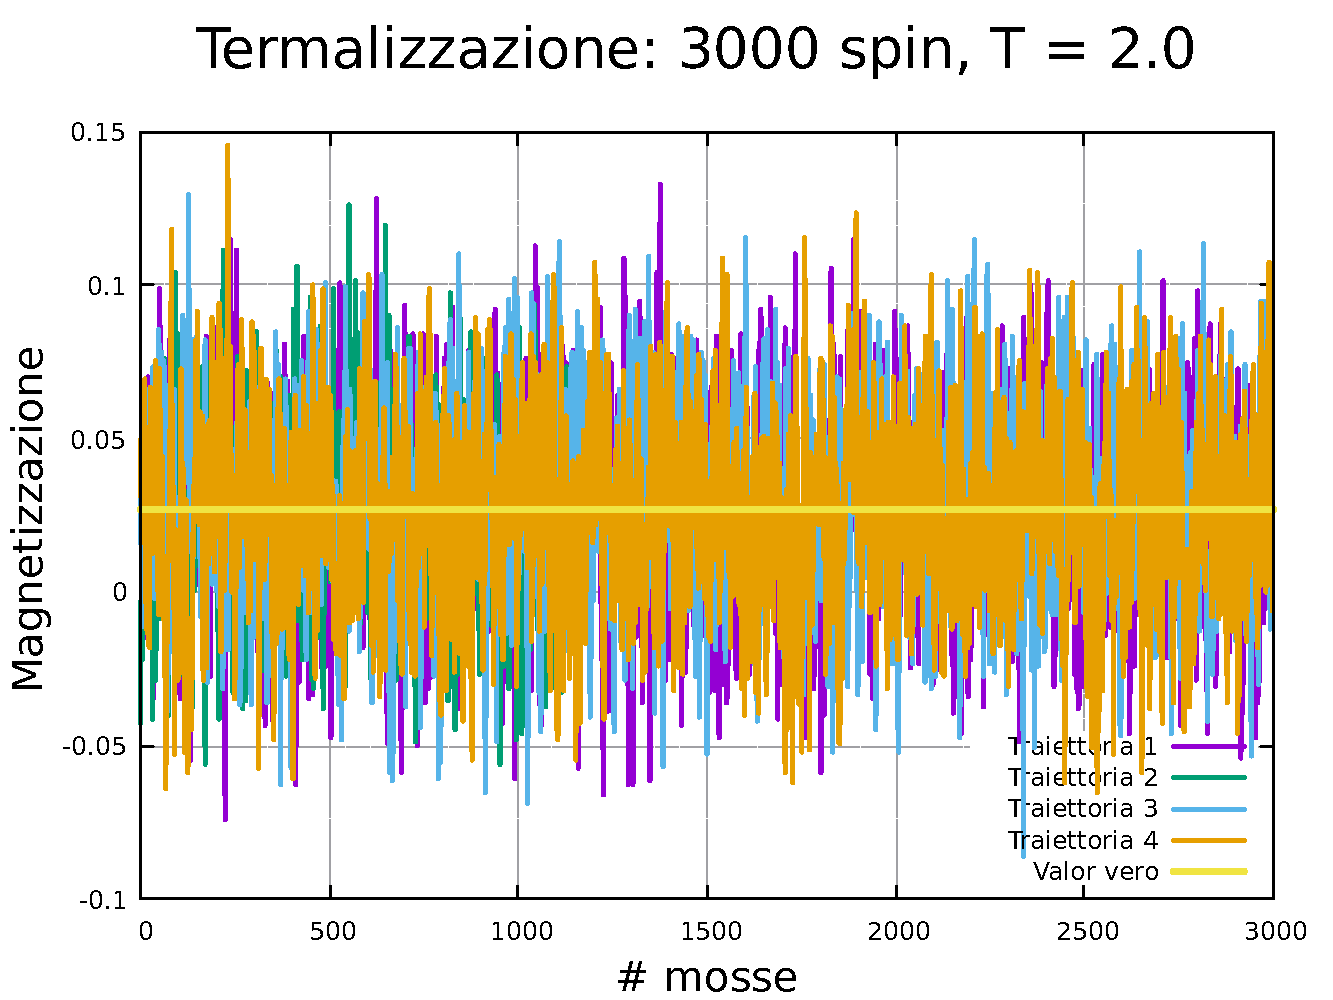
\includegraphics[page=1, width=\textwidth]{Immagini/simIsing1D/magn0.02/term/term_3000_2.0.pdf}
      \caption{$T\,=\,2.0$}
    \end{minipage}
    \caption{Studio della termalizzazione di un modello di Ising 1D costituito da 3000 spin.}
\end{figure}

\vspace*{\fill}

\newpage

\vspace*{\fill}

\begin{figure}[htbp]
    \centering
    \begin{minipage}{0.45\textwidth}  
      \centering
      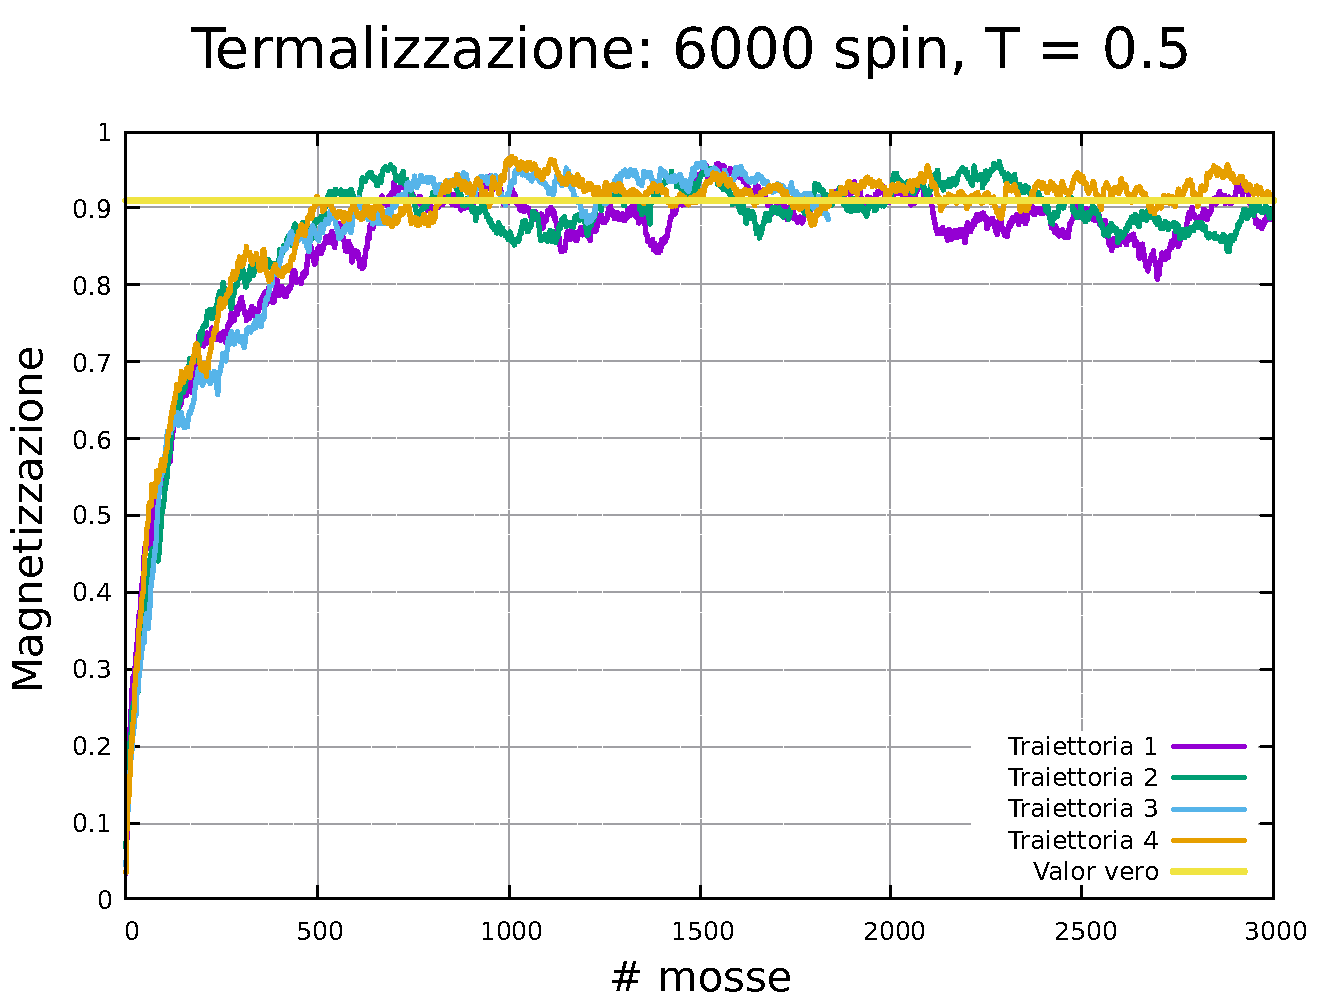
\includegraphics[page=1, width=\textwidth]{Immagini/simIsing1D/magn0.02/term/term_6000_0.5.pdf}
      \caption{$T\,=\,0.5$}
    \end{minipage}\hfill
    \begin{minipage}{0.45\textwidth}  
      \centering
      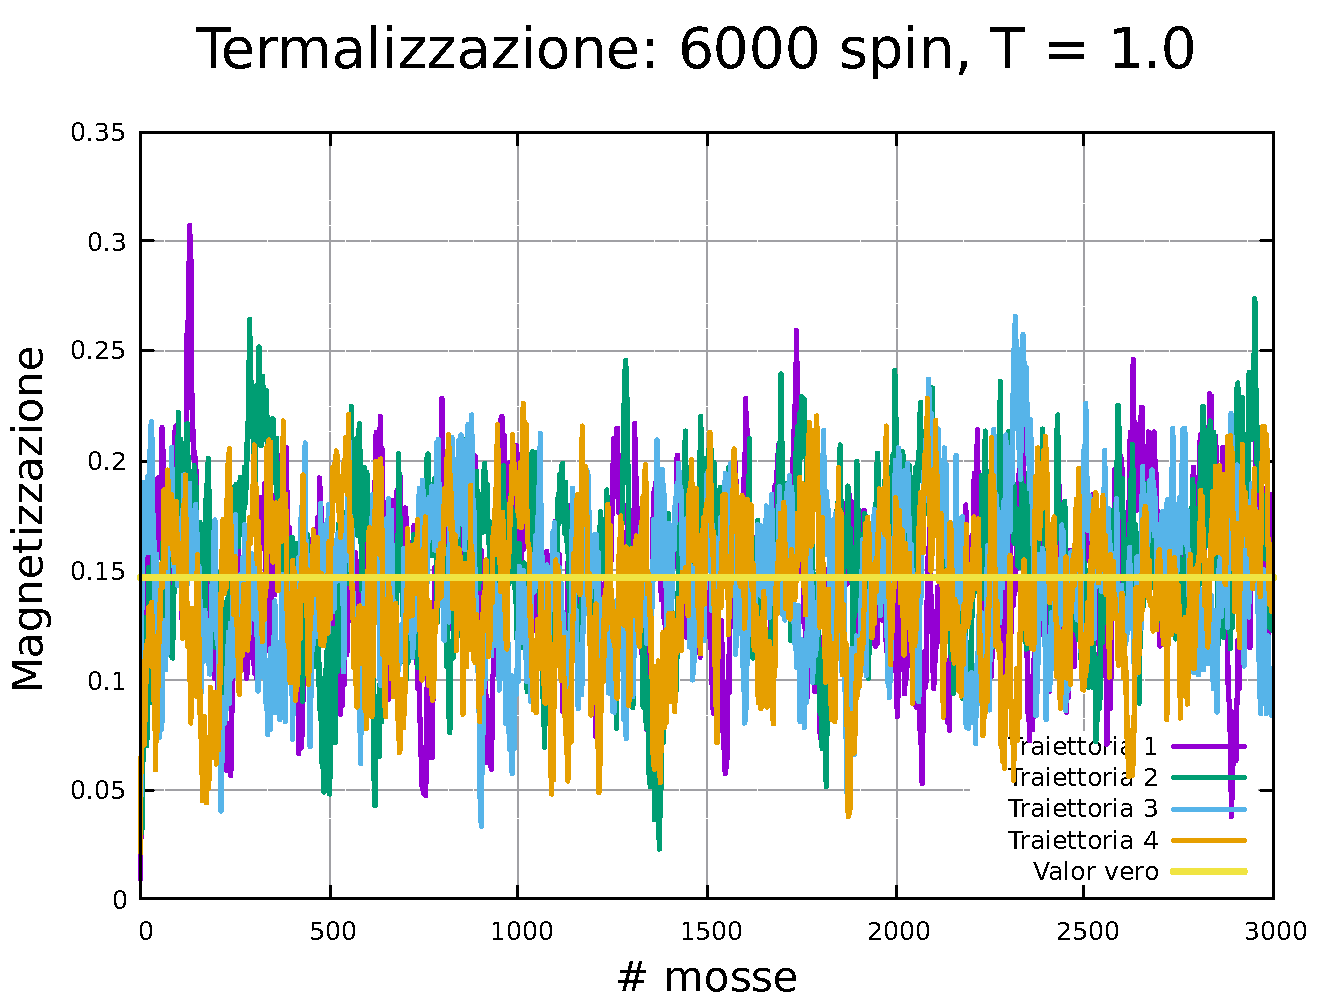
\includegraphics[page=1, width=\textwidth]{Immagini/simIsing1D/magn0.02/term/term_6000_1.0.pdf}
      \caption{$T\,=\,1.0$}
    \end{minipage}
    \vskip\baselineskip 
  
    \begin{minipage}{0.45\textwidth}  
      \centering
      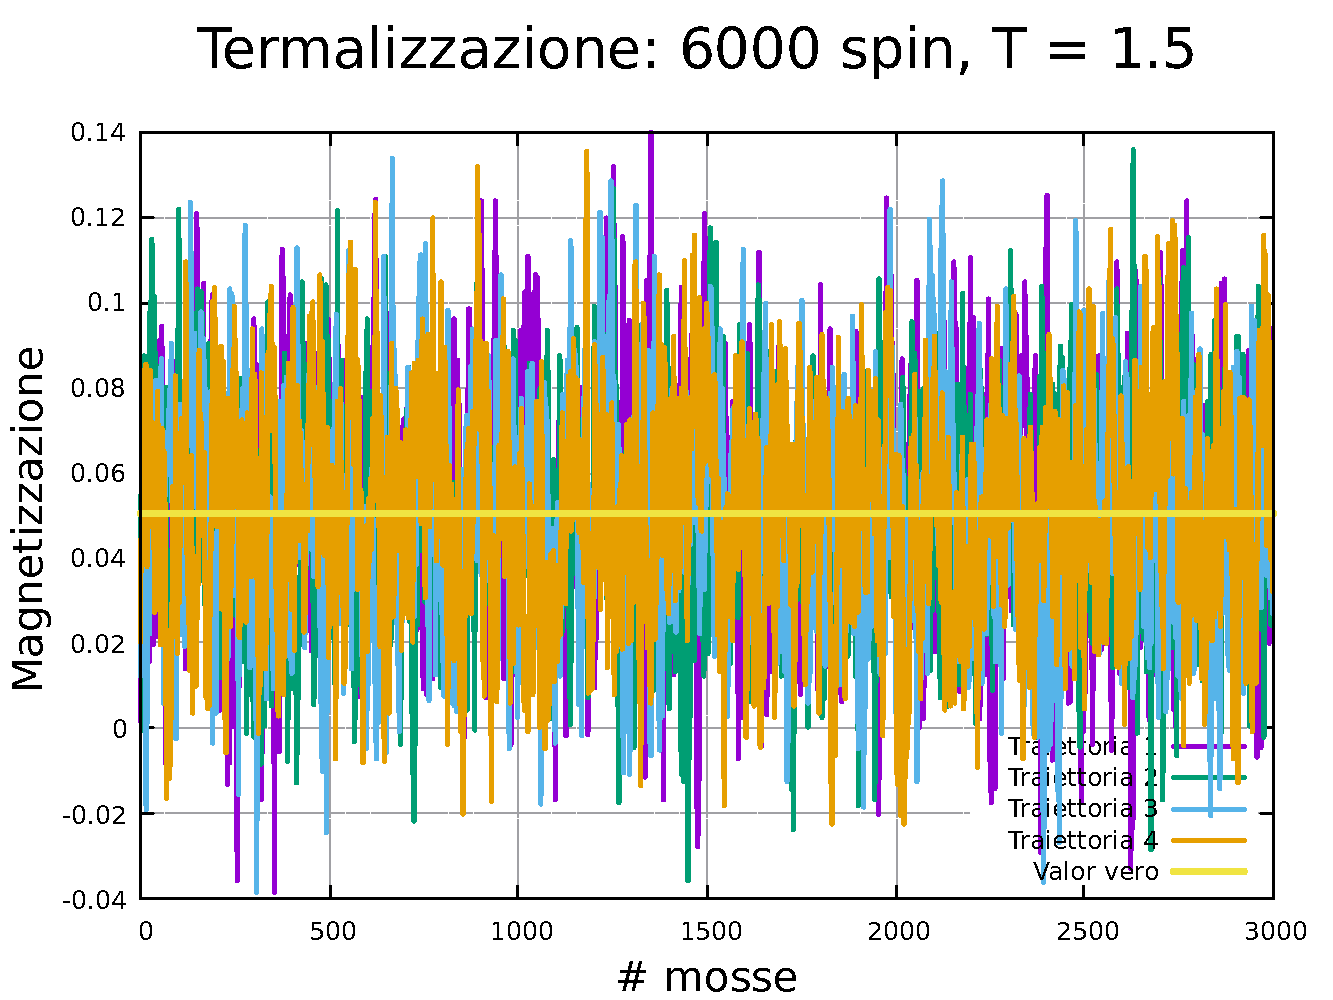
\includegraphics[page=1, width=\textwidth]{Immagini/simIsing1D/magn0.02/term/term_6000_1.5.pdf}
      \caption{$T\,=\,1.5$}
    \end{minipage}\hfill
    \begin{minipage}{0.45\textwidth}  
      \centering
      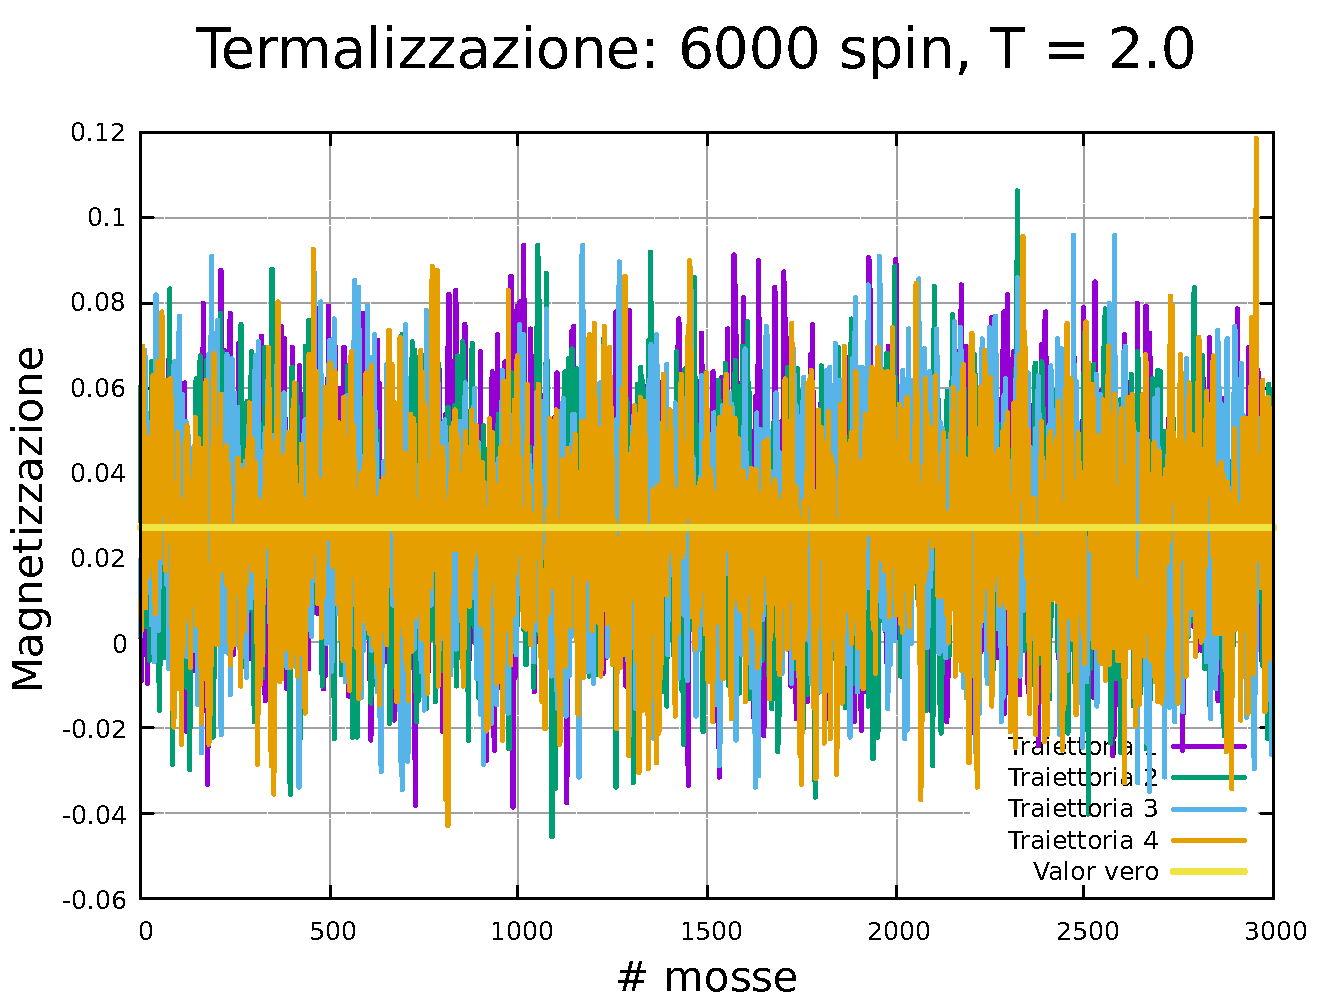
\includegraphics[page=1, width=\textwidth]{Immagini/simIsing1D/magn0.02/term/term_6000_2.0.pdf}
      \caption{$T\,=\,2.0$}
    \end{minipage}
    \caption{Studio della termalizzazione di un modello di Ising 1D costituito da 6000 spin.}
\end{figure}

\vspace*{\fill}

\newpage

\vspace*{\fill}

\begin{figure}[htbp]
    \centering
    \begin{minipage}{0.45\textwidth}  
      \centering
      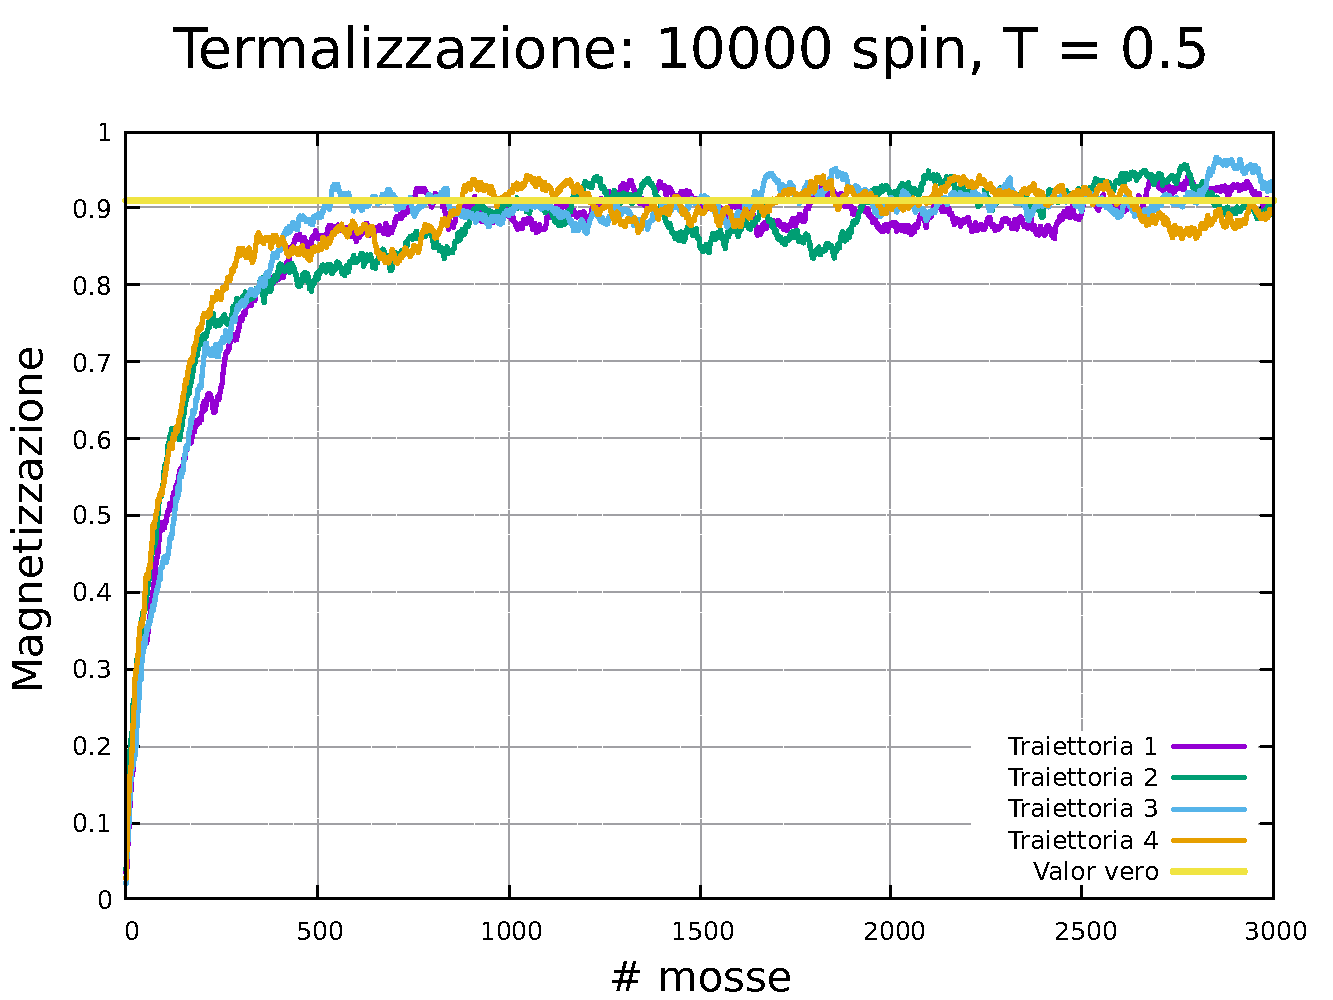
\includegraphics[page=1, width=\textwidth]{Immagini/simIsing1D/magn0.02/term/term_10000_0.5.pdf}
      \caption{$T\,=\,0.5$}
    \end{minipage}\hfill
    \begin{minipage}{0.45\textwidth}  
      \centering
      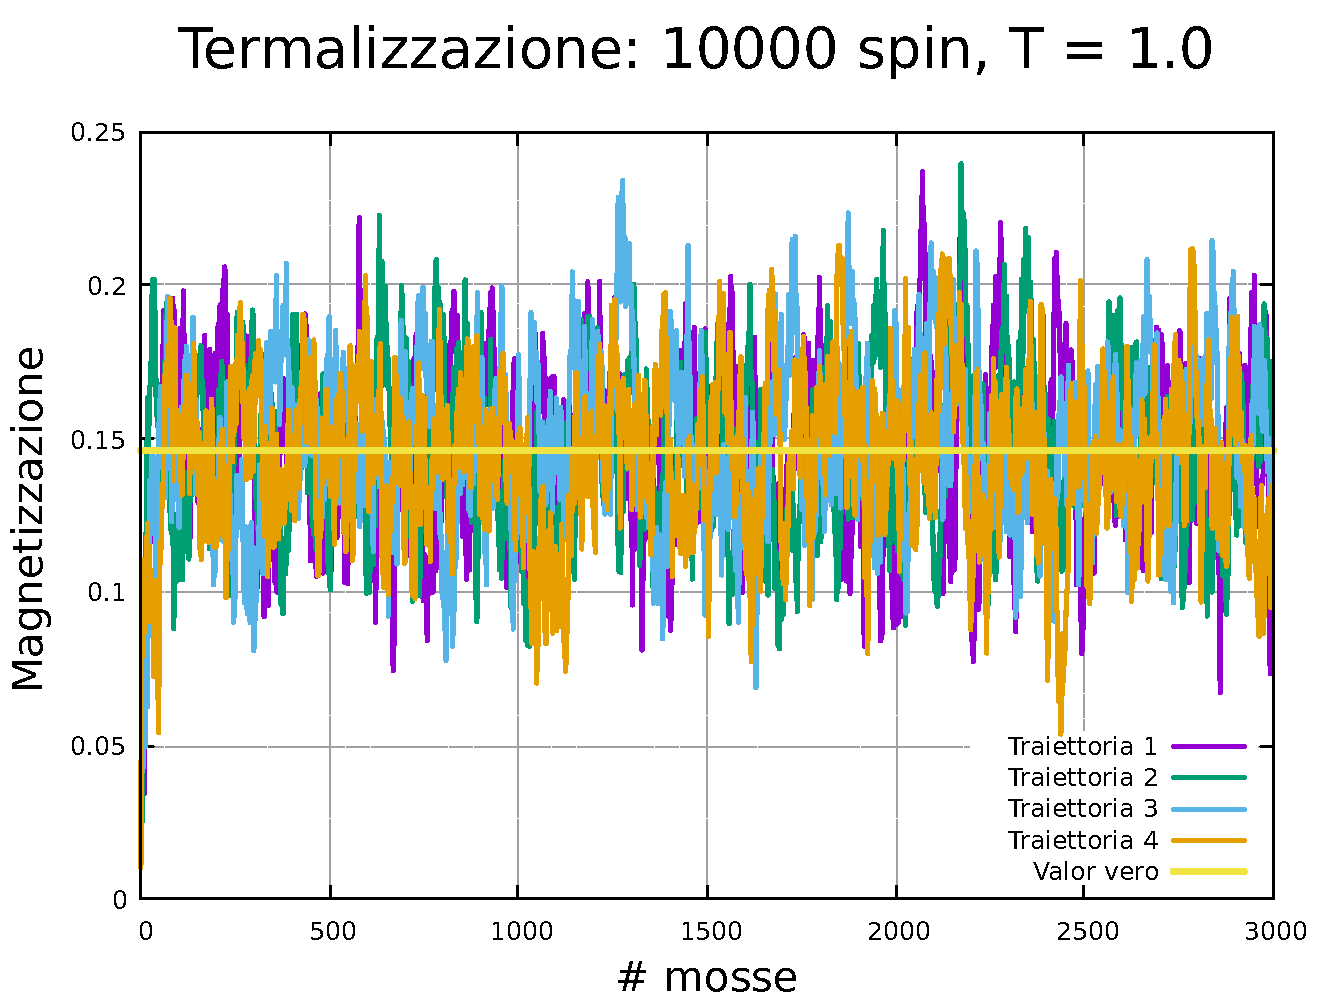
\includegraphics[page=1, width=\textwidth]{Immagini/simIsing1D/magn0.02/term/term_10000_1.0.pdf}
      \caption{$T\,=\,1.0$}
    \end{minipage}
    \vskip\baselineskip 
  
    \begin{minipage}{0.45\textwidth}  
      \centering
      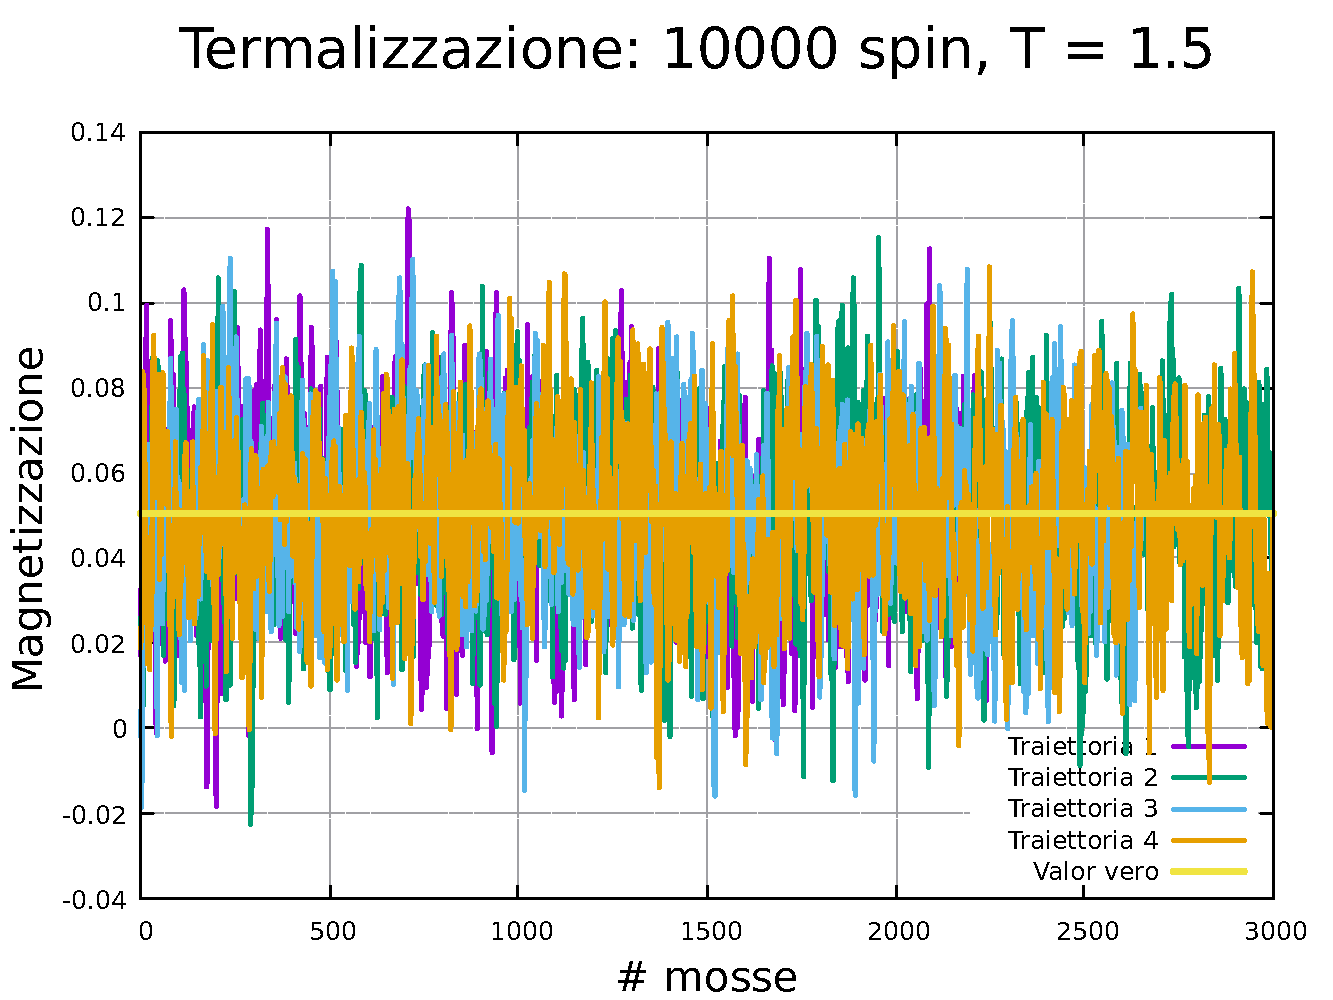
\includegraphics[page=1, width=\textwidth]{Immagini/simIsing1D/magn0.02/term/term_10000_1.5.pdf}
      \caption{$T\,=\,1.5$}
    \end{minipage}\hfill
    \begin{minipage}{0.45\textwidth}  
      \centering
      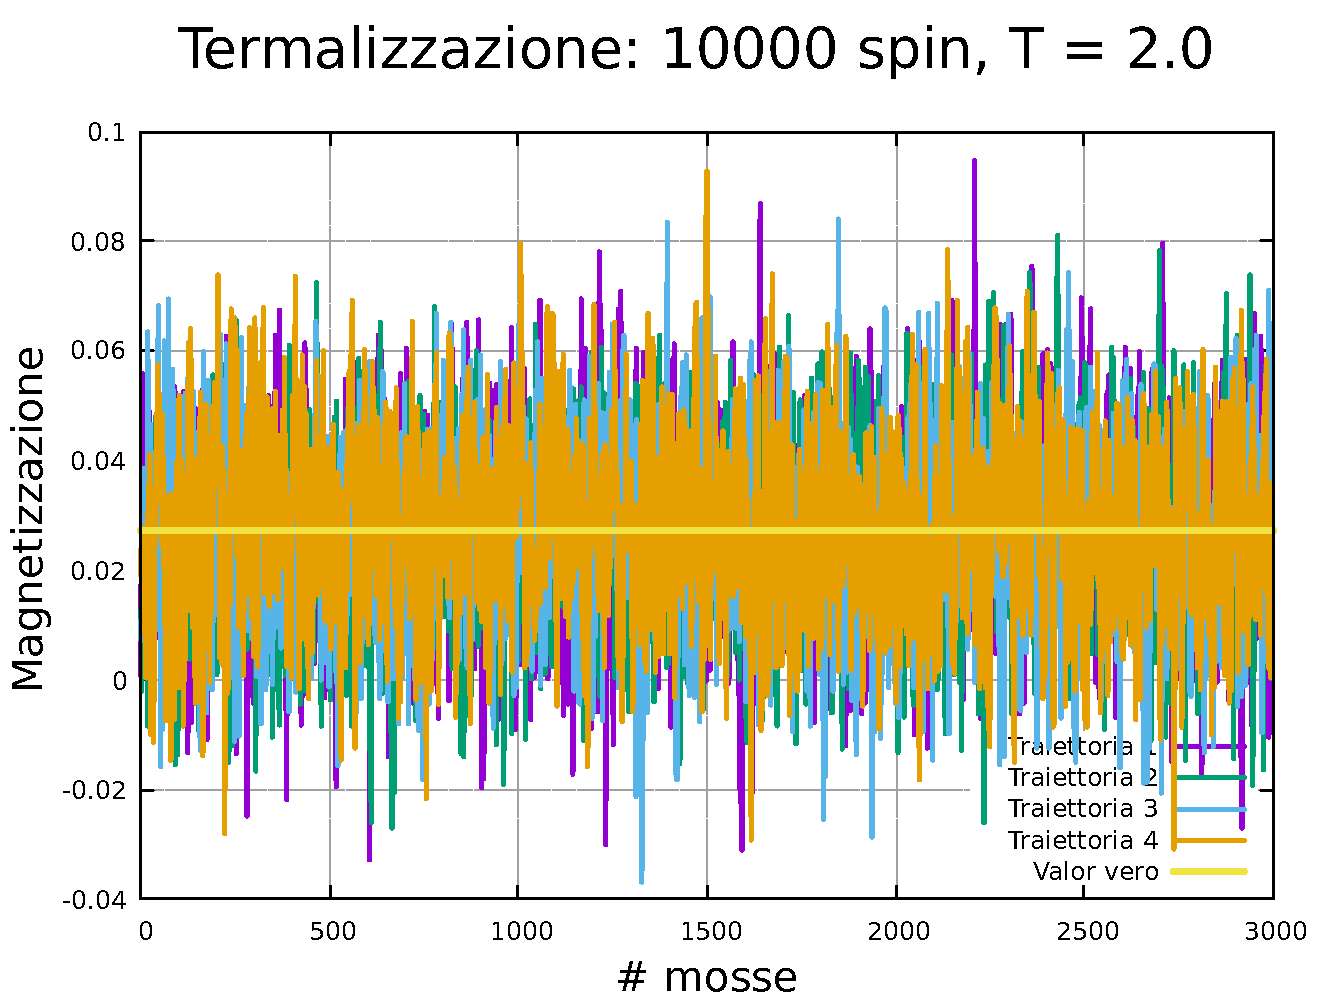
\includegraphics[page=1, width=\textwidth]{Immagini/simIsing1D/magn0.02/term/term_10000_2.0.pdf}
      \caption{$T\,=\,2.0$}
    \end{minipage}
    \caption{Studio della termalizzazione di un modello di Ising 1D costituito da 10000 spin.}
\end{figure}

\vspace*{\fill}

\newpage



\subsubsection{Auto-correlazione}

\vspace*{\fill}

\begin{figure}[htbp]
    \centering
    \begin{minipage}{0.45\textwidth}  
      \centering
      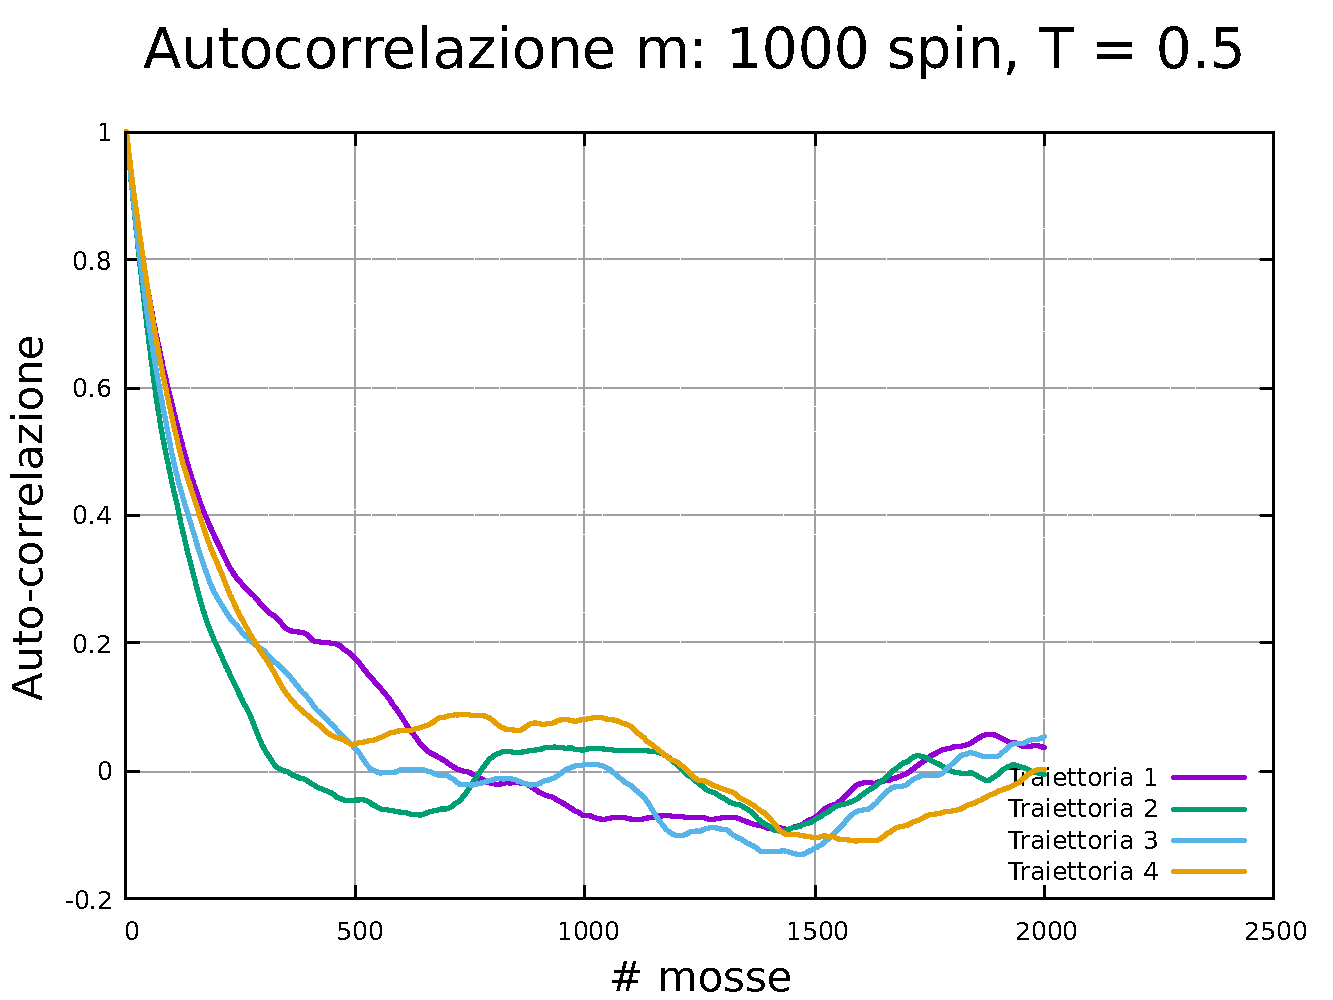
\includegraphics[page=1, width=\textwidth]{Immagini/simIsing1D/magn0.02/tcorr/tcorr_1000_0.5.pdf}
      \caption{$T\,=\,0.5$}
    \end{minipage}\hfill
    \begin{minipage}{0.45\textwidth}  
      \centering
      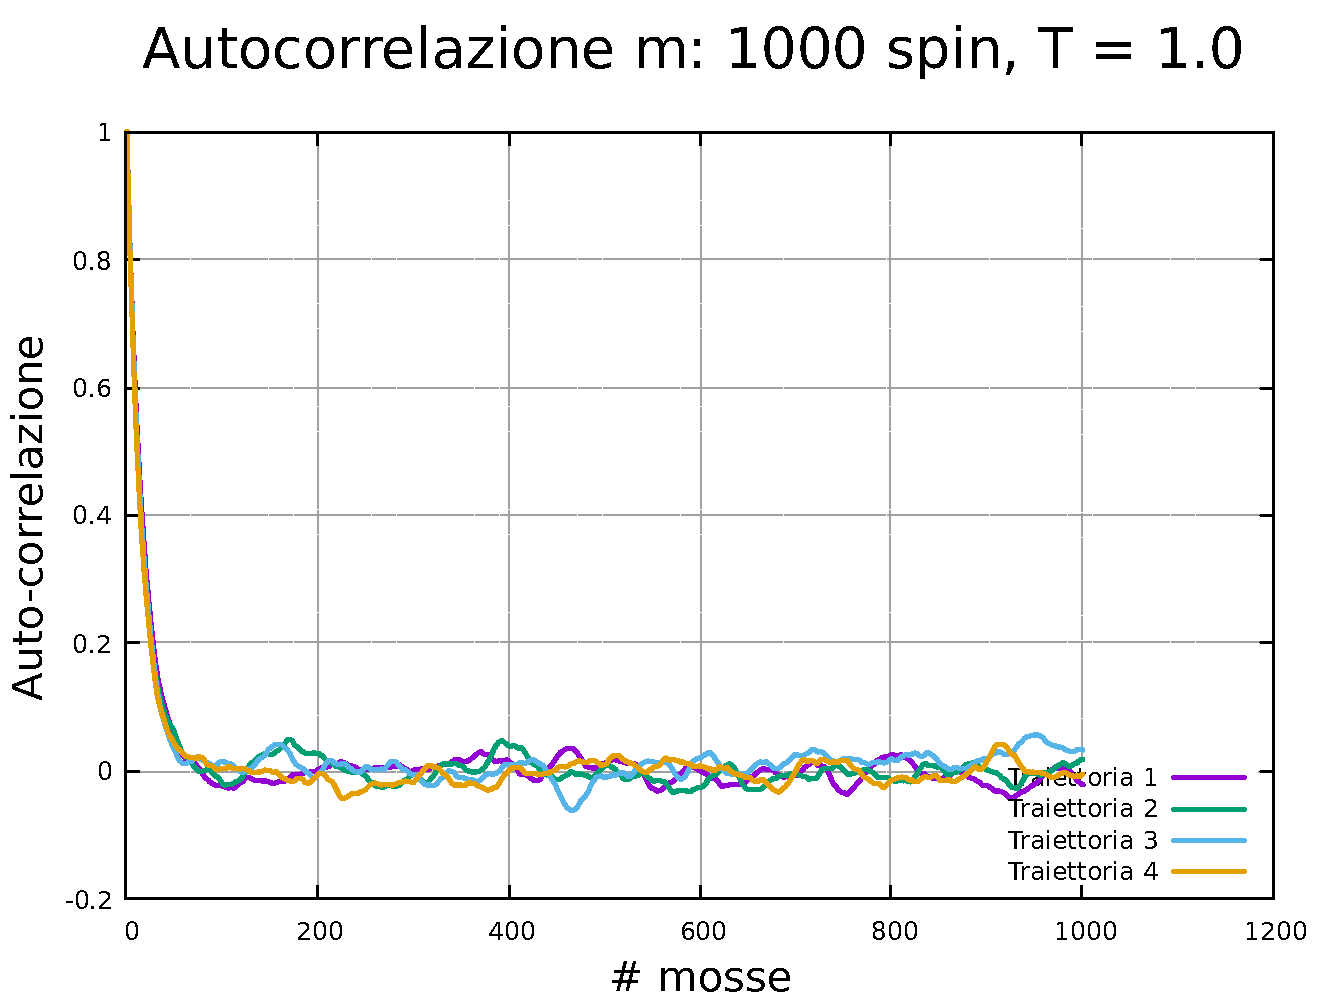
\includegraphics[page=1, width=\textwidth]{Immagini/simIsing1D/magn0.02/tcorr/tcorr_1000_1.0.pdf}
      \caption{$T\,=\,1.0$}
    \end{minipage}
    \vskip\baselineskip 
  
    \begin{minipage}{0.45\textwidth}  
      \centering
      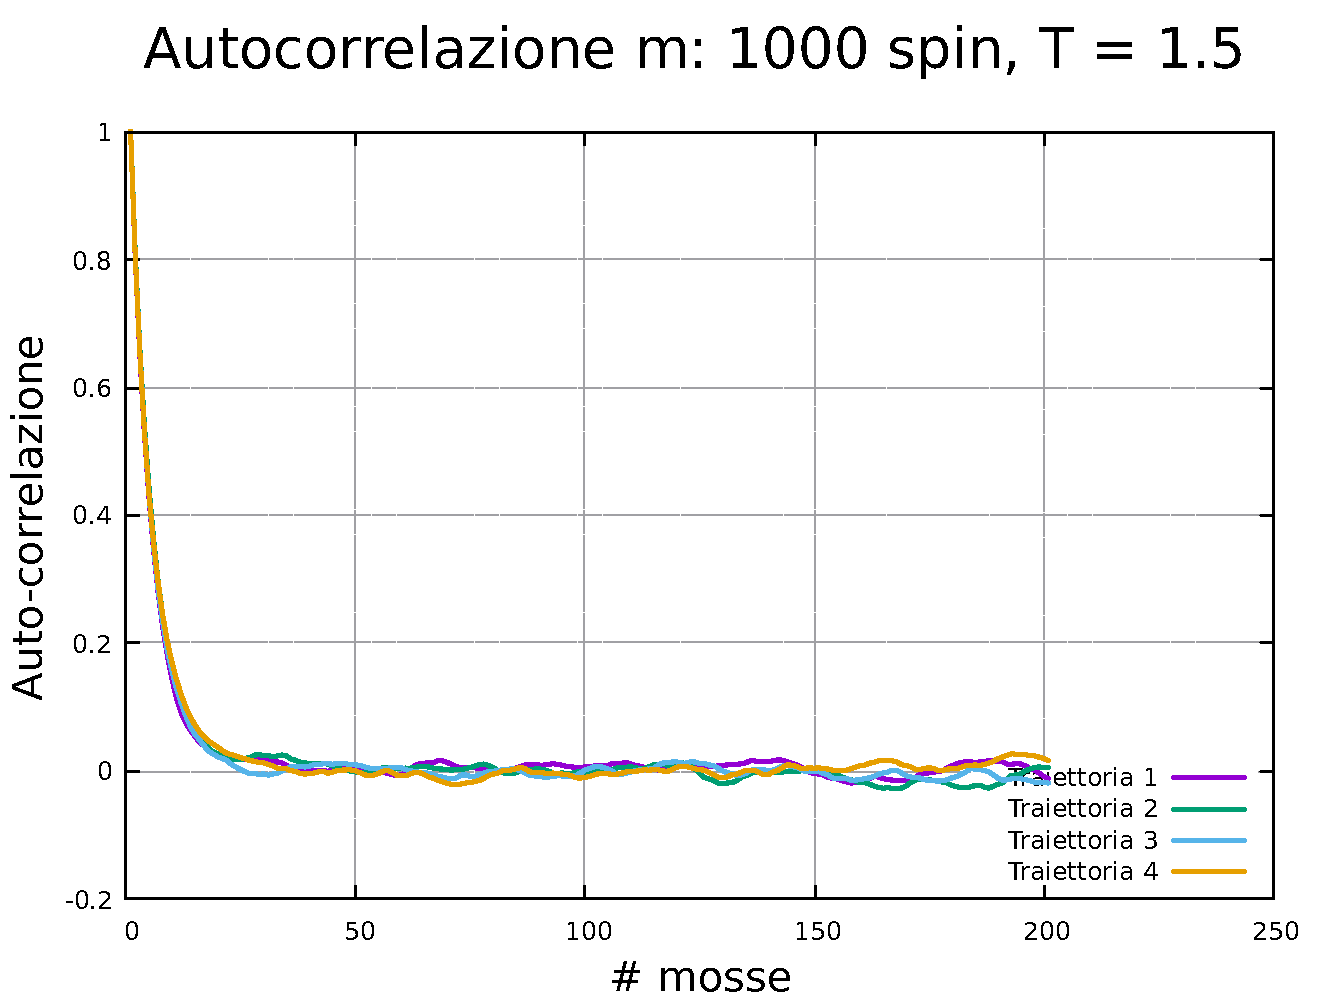
\includegraphics[page=1, width=\textwidth]{Immagini/simIsing1D/magn0.02/tcorr/tcorr_1000_1.5.pdf}
      \caption{$T\,=\,1.5$}
    \end{minipage}\hfill
    \begin{minipage}{0.45\textwidth}  
      \centering
      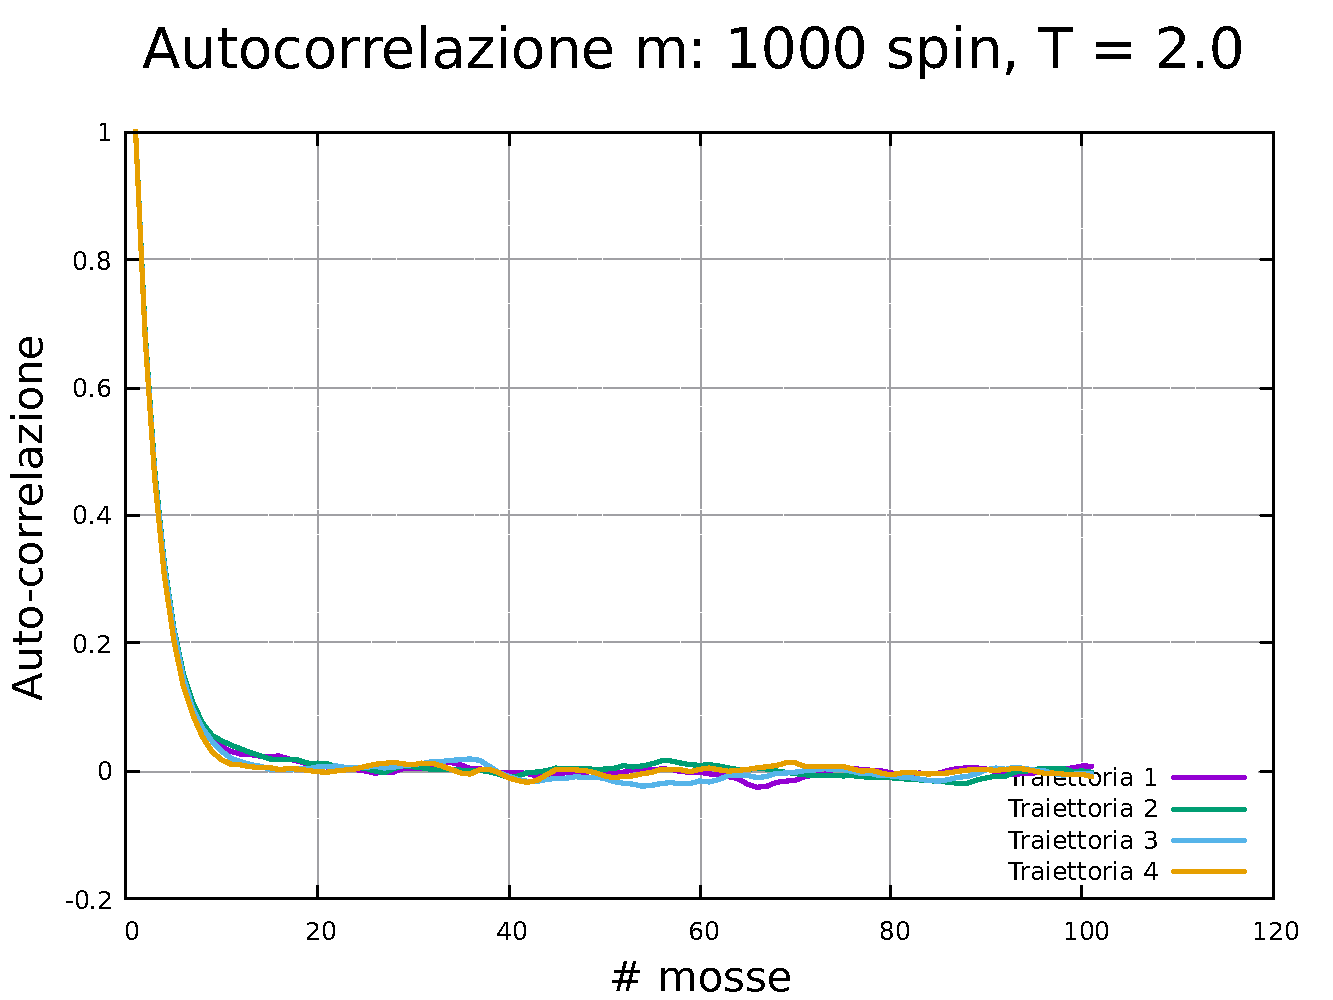
\includegraphics[page=1, width=\textwidth]{Immagini/simIsing1D/magn0.02/tcorr/tcorr_1000_2.0.pdf}
      \caption{$T\,=\,2.0$}
    \end{minipage}
    \caption{Studio dell'auto-correlazione per un modello di Ising 1D costituito da 1000 spin.}
\end{figure}

\vspace*{\fill}

\newpage

\vspace*{\fill}

\begin{figure}[htbp]
    \centering
    \begin{minipage}{0.45\textwidth}  
      \centering
      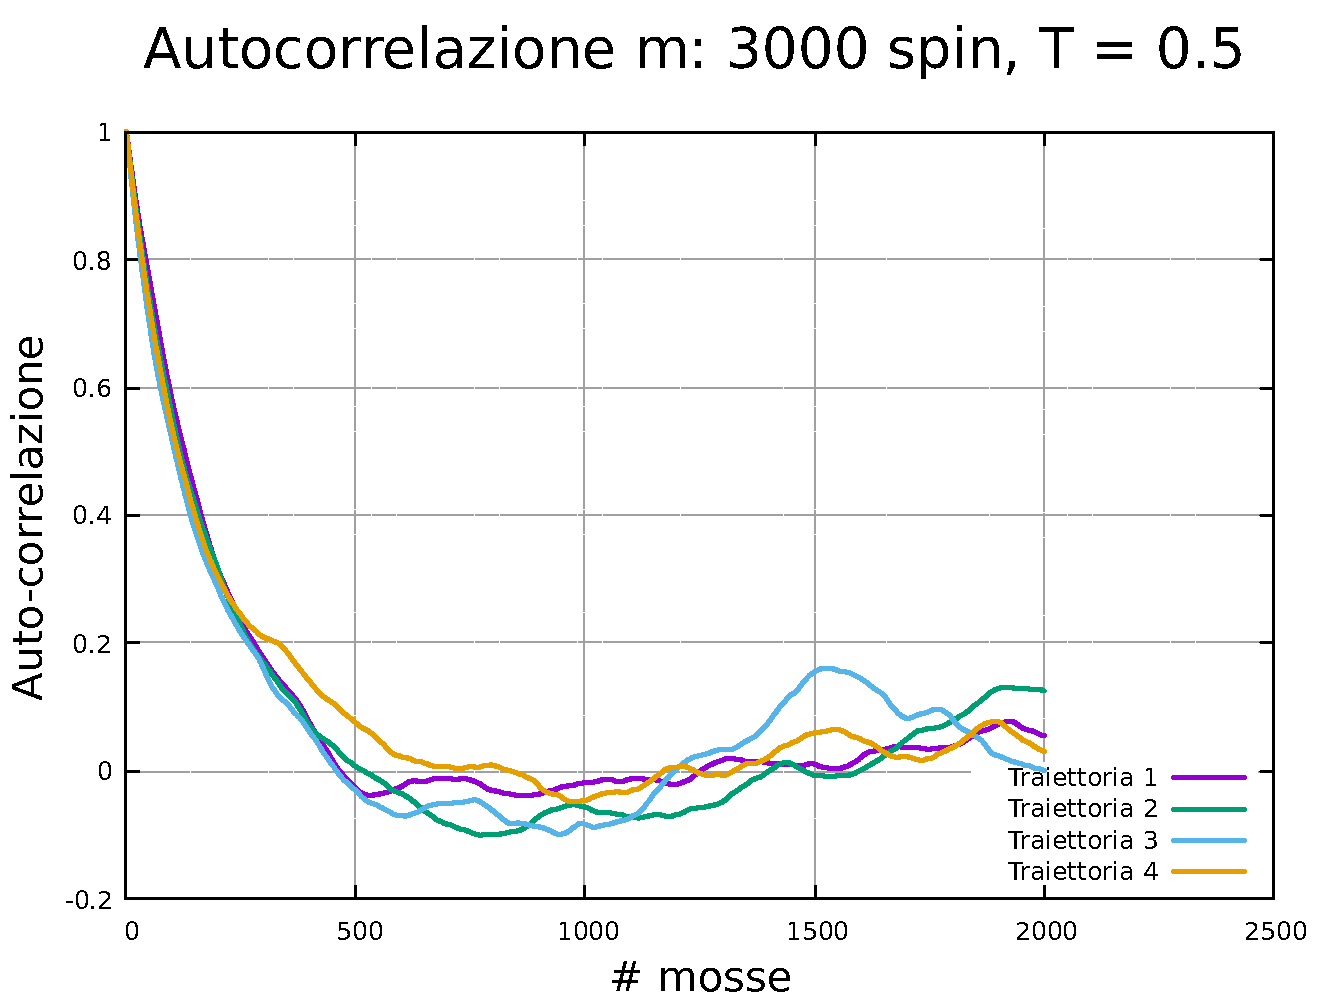
\includegraphics[page=1, width=\textwidth]{Immagini/simIsing1D/magn0.02/tcorr/tcorr_3000_0.5.pdf}
      \caption{$T\,=\,0.5$}
    \end{minipage}\hfill
    \begin{minipage}{0.45\textwidth}  
      \centering
      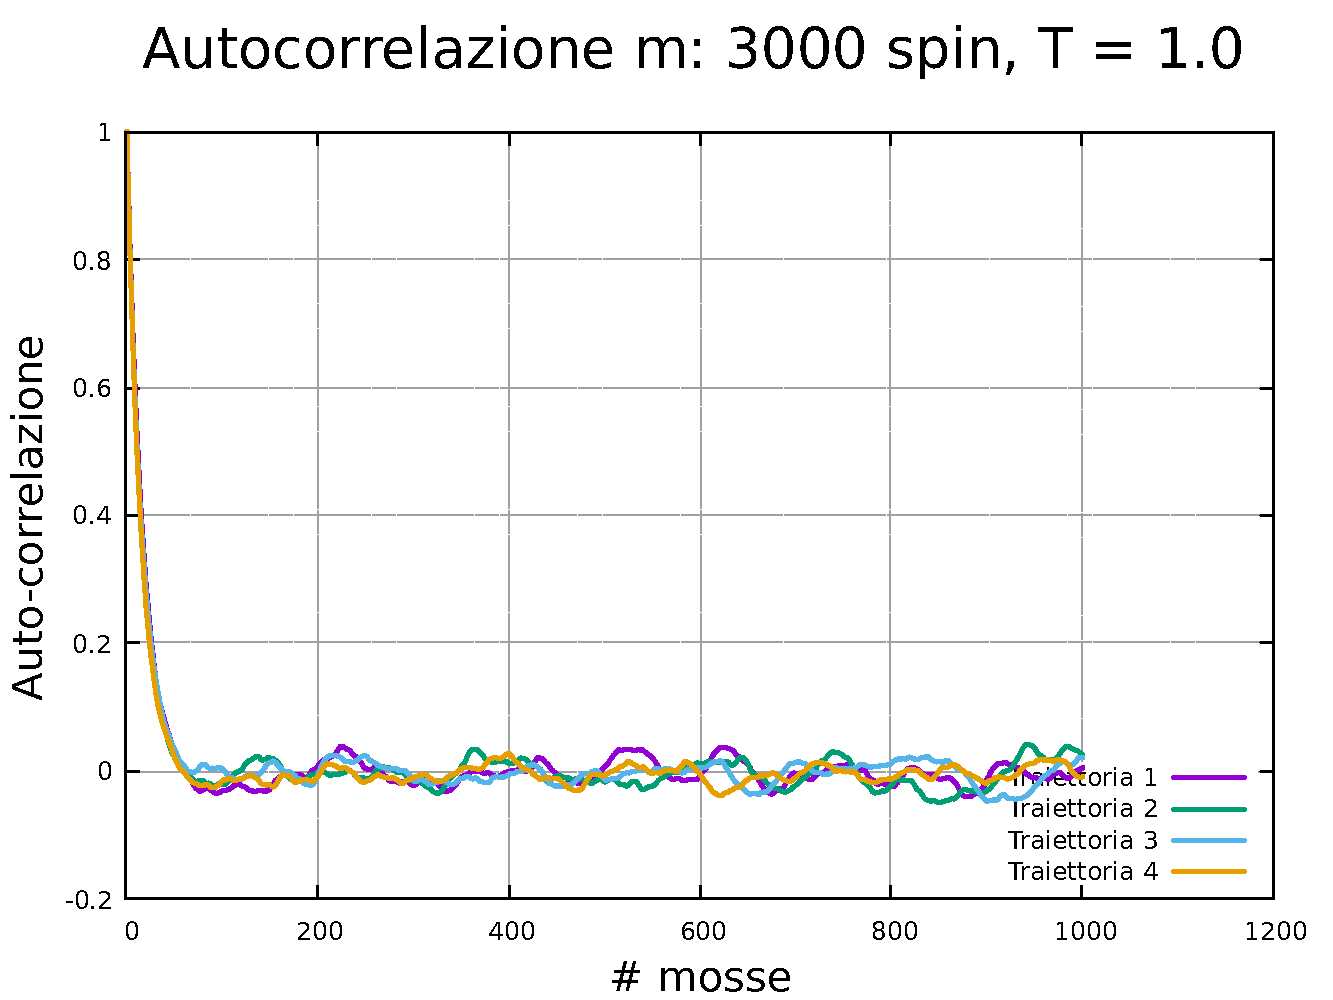
\includegraphics[page=1, width=\textwidth]{Immagini/simIsing1D/magn0.02/tcorr/tcorr_3000_1.0.pdf}
      \caption{$T\,=\,1.0$}
    \end{minipage}
    \vskip\baselineskip 
  
    \begin{minipage}{0.45\textwidth}  
      \centering
      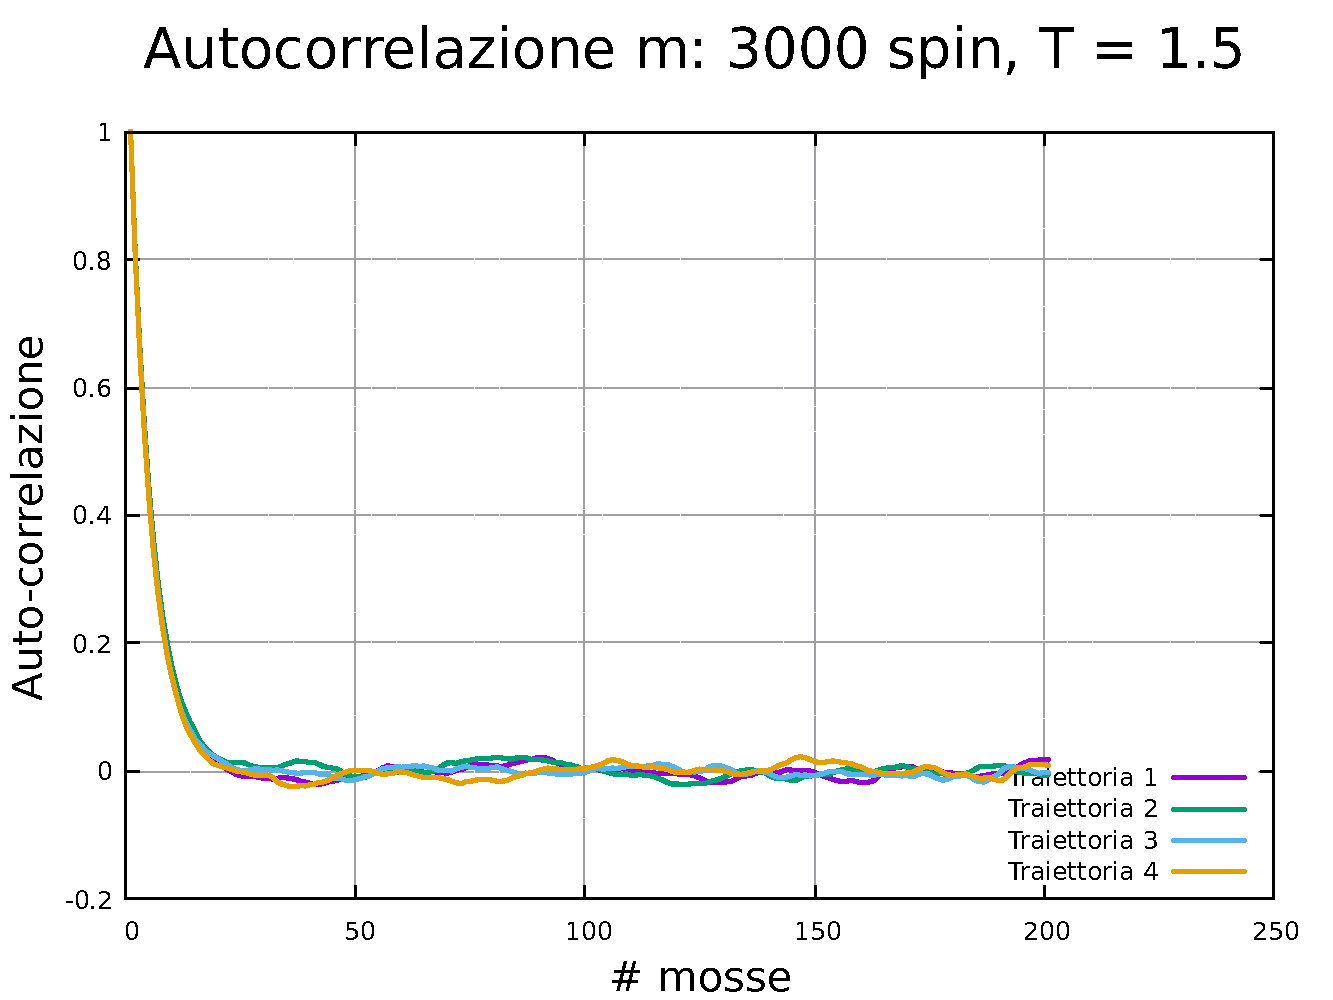
\includegraphics[page=1, width=\textwidth]{Immagini/simIsing1D/magn0.02/tcorr/tcorr_3000_1.5.pdf}
      \caption{$T\,=\,1.5$}
    \end{minipage}\hfill
    \begin{minipage}{0.45\textwidth}  
      \centering
      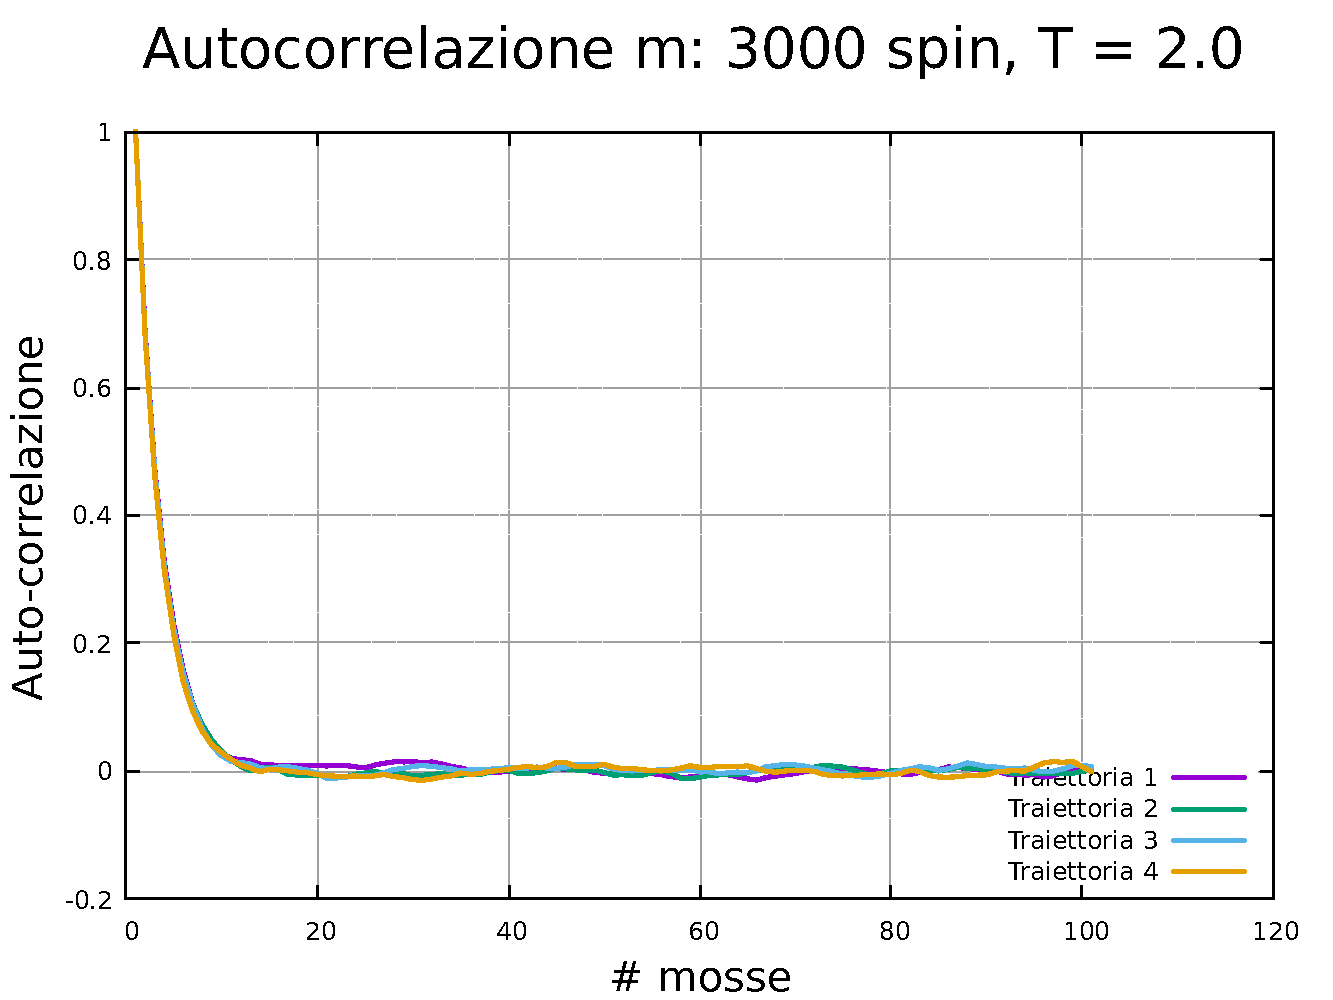
\includegraphics[page=1, width=\textwidth]{Immagini/simIsing1D/magn0.02/tcorr/tcorr_3000_2.0.pdf}
      \caption{$T\,=\,2.0$}
    \end{minipage}
    \caption{Studio dell'auto-correlazione per un modello di Ising 1D costituito da 3000 spin.}
\end{figure}

\vspace*{\fill}

\newpage

\vspace*{\fill}

\begin{figure}[htbp]
    \centering
    \begin{minipage}{0.45\textwidth}  
      \centering
      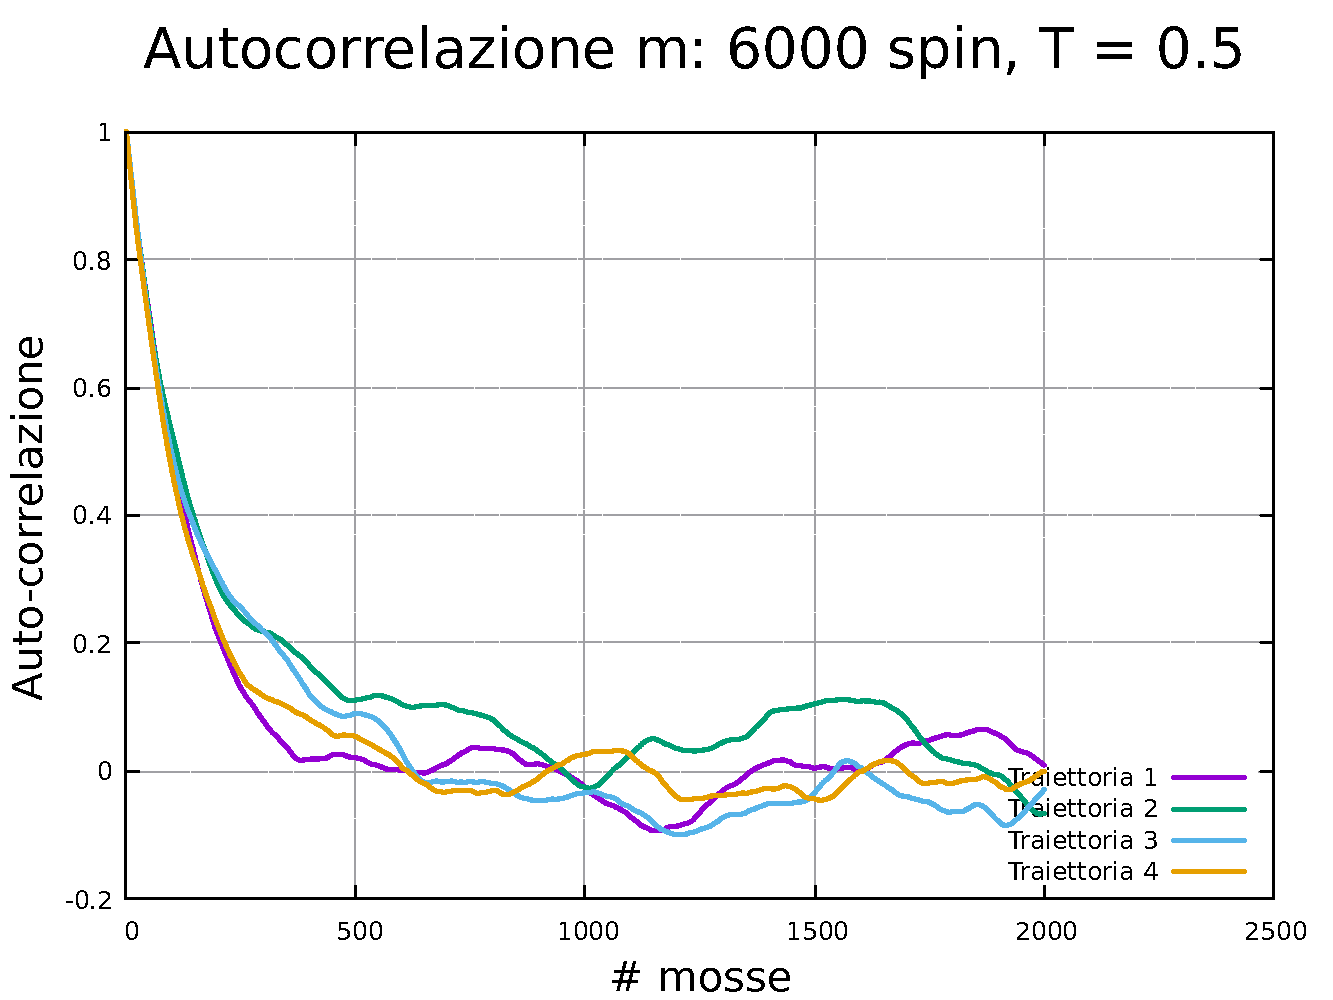
\includegraphics[page=1, width=\textwidth]{Immagini/simIsing1D/magn0.02/tcorr/tcorr_6000_0.5.pdf}
      \caption{$T\,=\,0.5$}
    \end{minipage}\hfill
    \begin{minipage}{0.45\textwidth}  
      \centering
      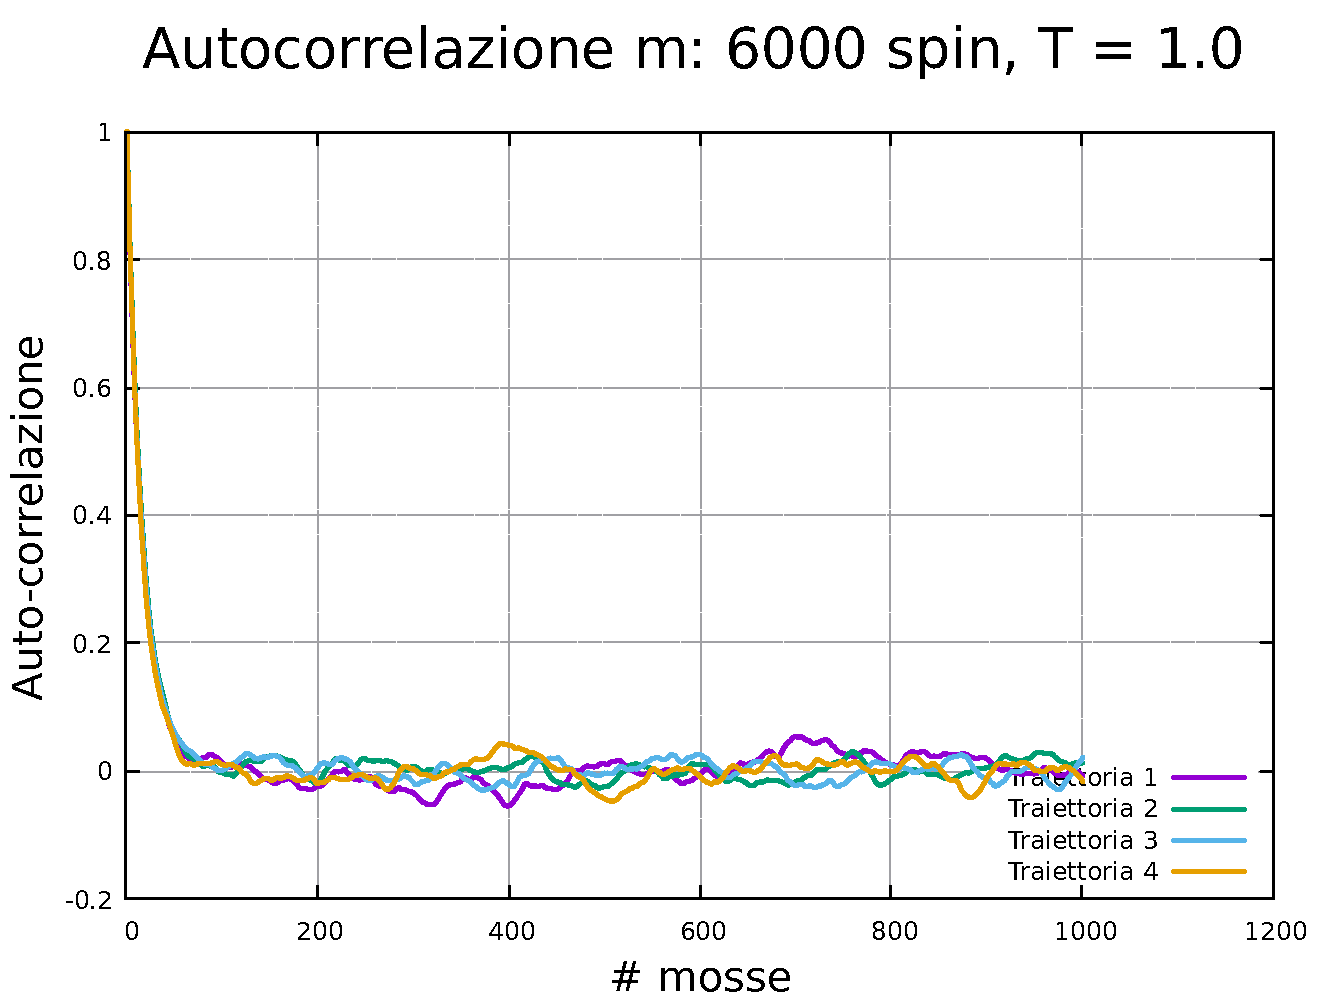
\includegraphics[page=1, width=\textwidth]{Immagini/simIsing1D/magn0.02/tcorr/tcorr_6000_1.0.pdf}
      \caption{$T\,=\,1.0$}
    \end{minipage}
    \vskip\baselineskip 
  
    \begin{minipage}{0.45\textwidth}  
      \centering
      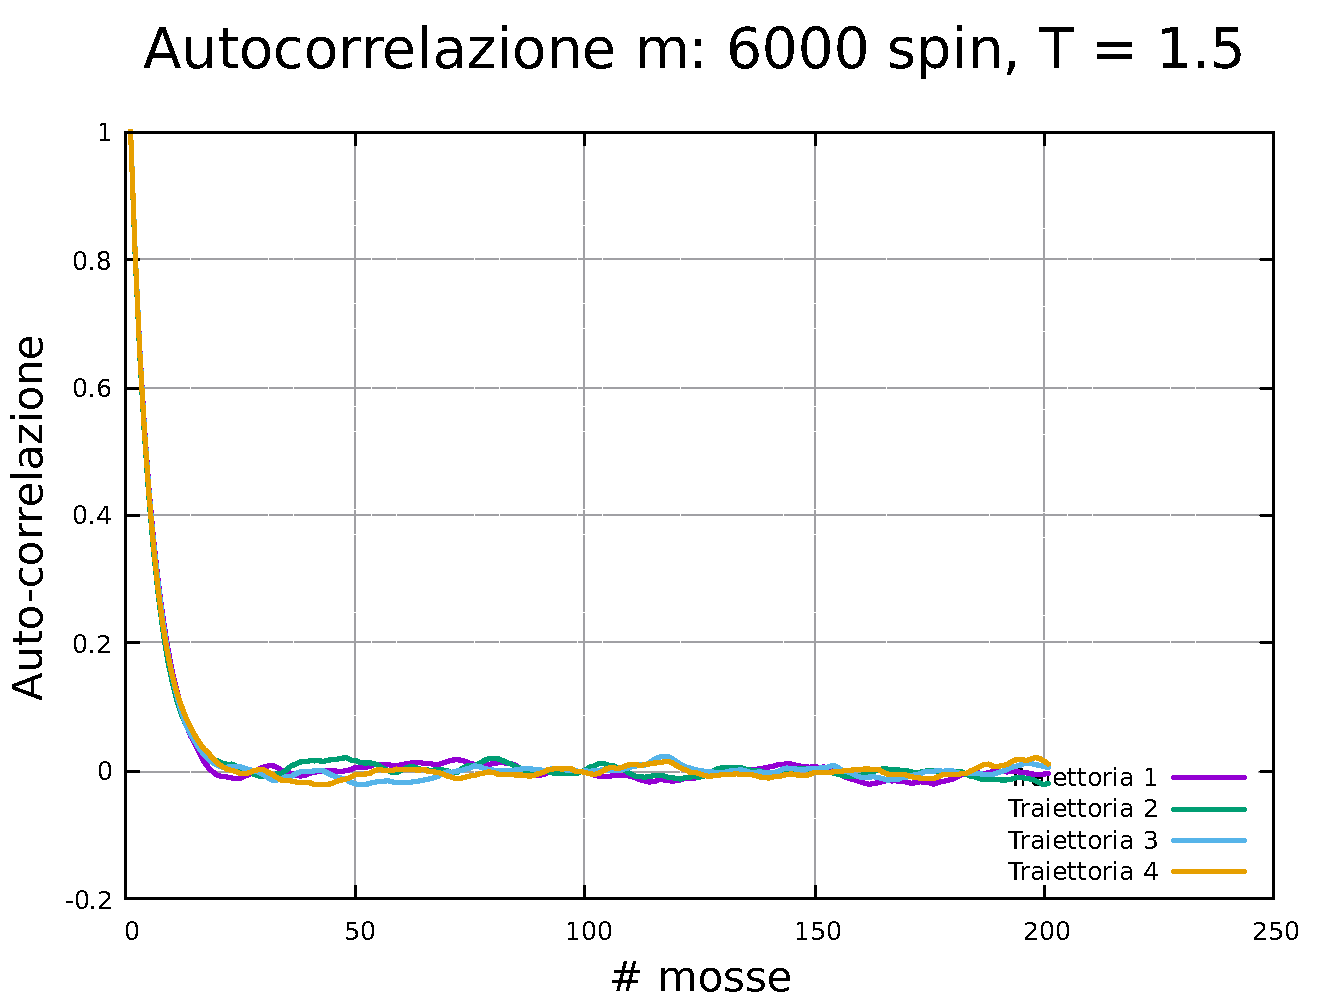
\includegraphics[page=1, width=\textwidth]{Immagini/simIsing1D/magn0.02/tcorr/tcorr_6000_1.5.pdf}
      \caption{$T\,=\,1.5$}
    \end{minipage}\hfill
    \begin{minipage}{0.45\textwidth}  
      \centering
      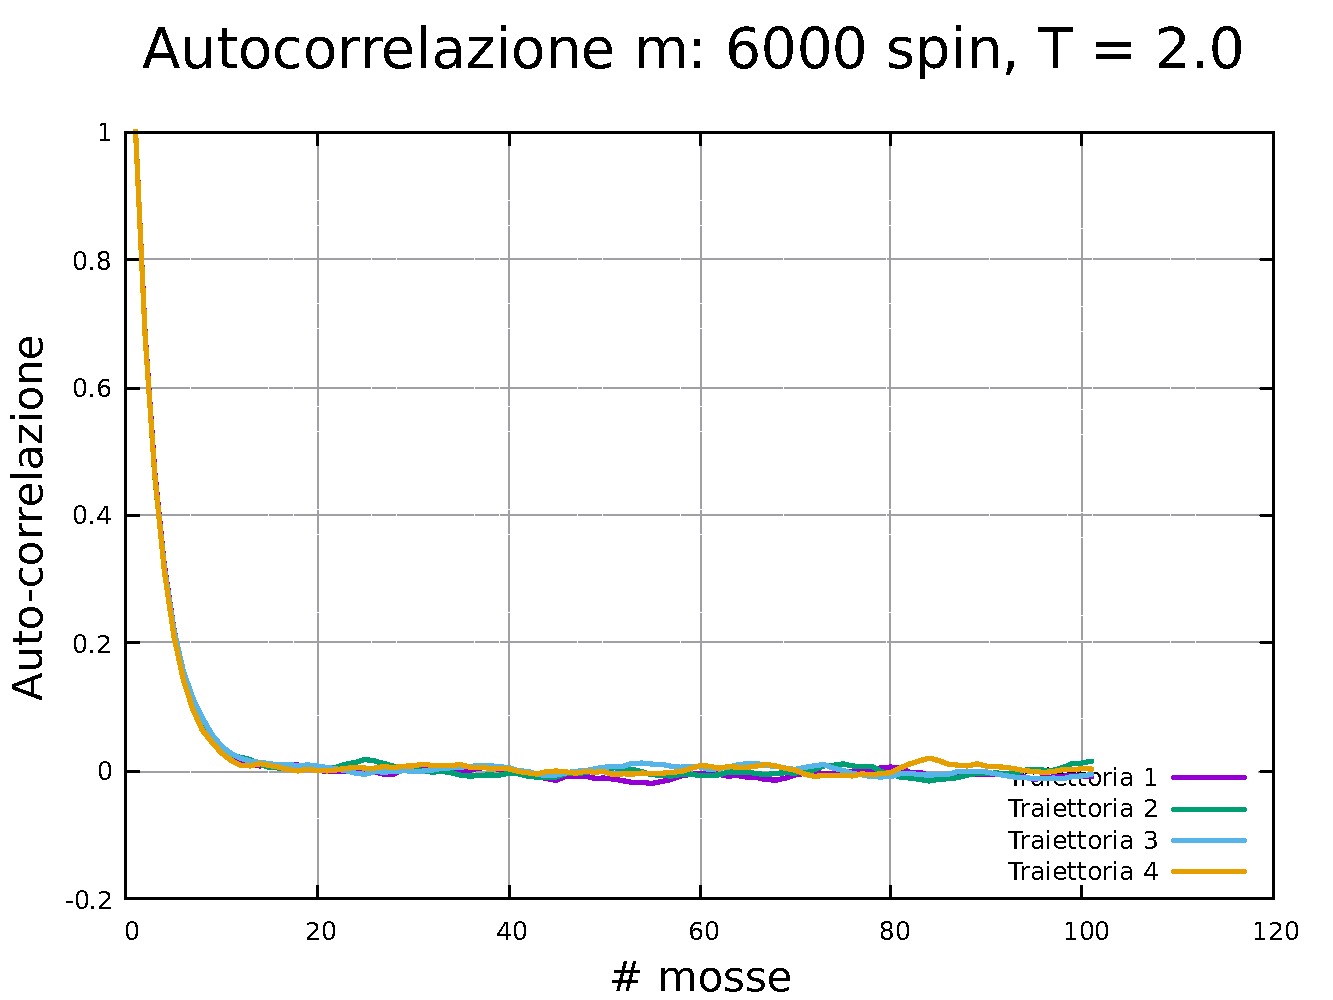
\includegraphics[page=1, width=\textwidth]{Immagini/simIsing1D/magn0.02/tcorr/tcorr_6000_2.0.pdf}
      \caption{$T\,=\,2.0$}
    \end{minipage}
    \caption{Studio dell'auto-correlazione per un modello di Ising 1D costituito da 6000 spin.}
\end{figure}

\vspace*{\fill}

\newpage

\vspace*{\fill}

\begin{figure}[htbp]
    \centering
    \begin{minipage}{0.45\textwidth}  
      \centering
      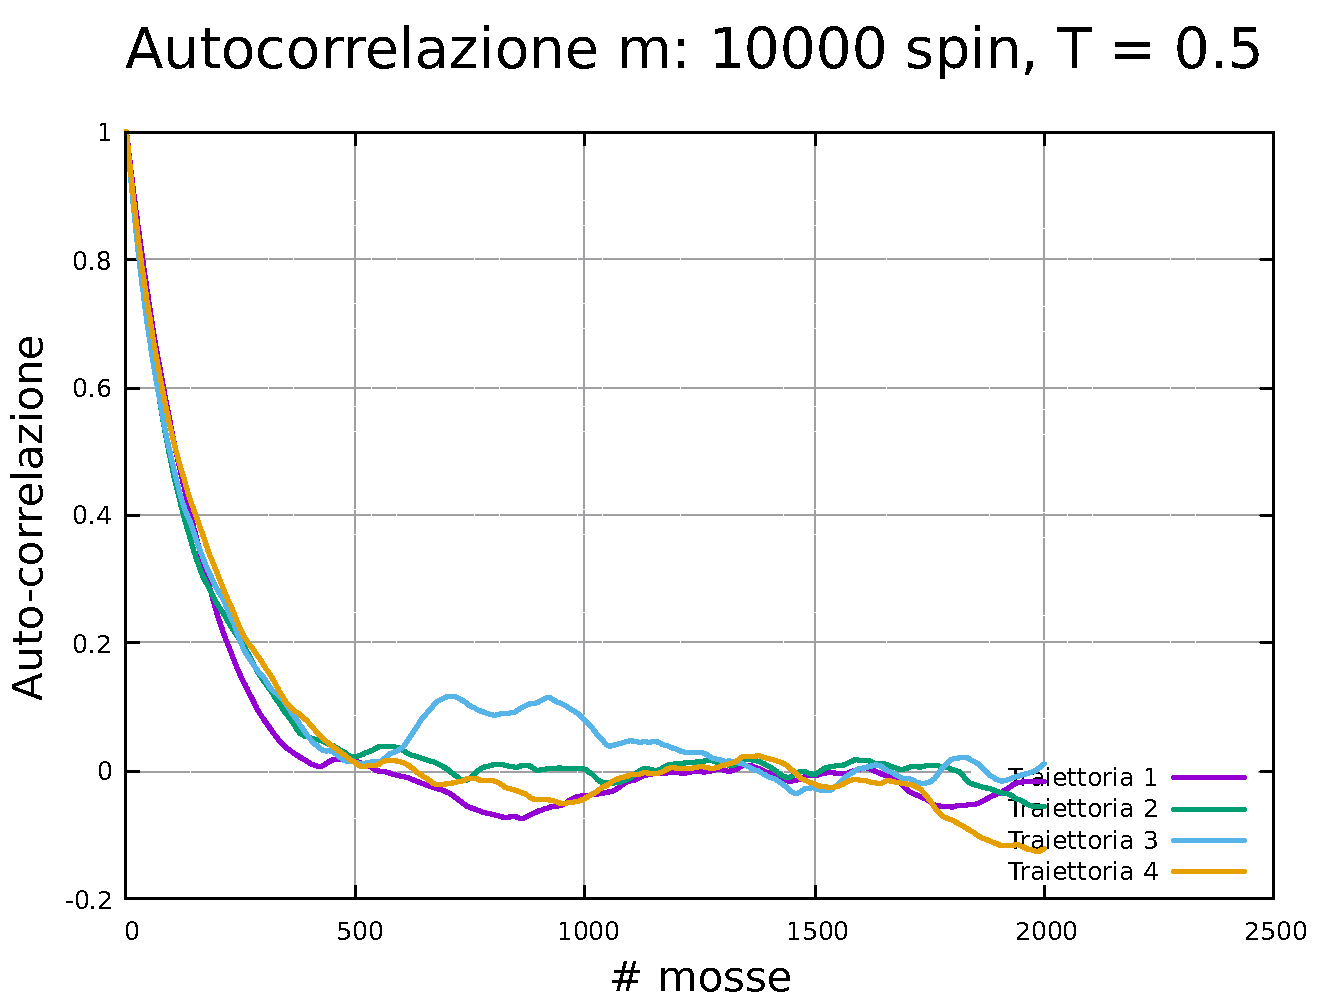
\includegraphics[page=1, width=\textwidth]{Immagini/simIsing1D/magn0.02/tcorr/tcorr_10000_0.5.pdf}
      \caption{$T\,=\,0.5$}
    \end{minipage}\hfill
    \begin{minipage}{0.45\textwidth}  
      \centering
      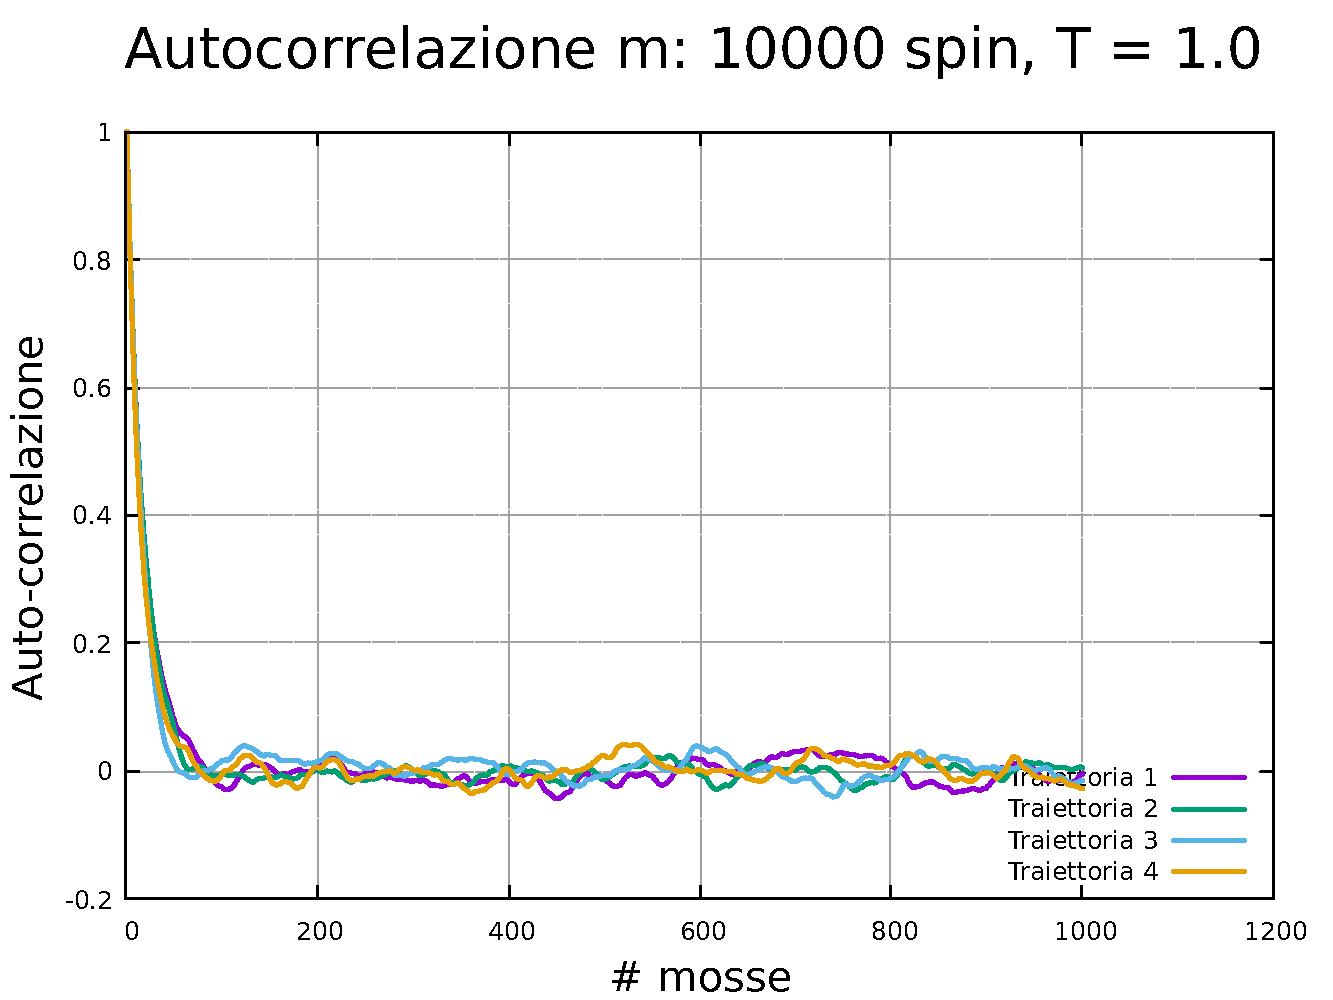
\includegraphics[page=1, width=\textwidth]{Immagini/simIsing1D/magn0.02/tcorr/tcorr_10000_1.0.pdf}
      \caption{$T\,=\,1.0$}
    \end{minipage}
    \vskip\baselineskip 
  
    \begin{minipage}{0.45\textwidth}  
      \centering
      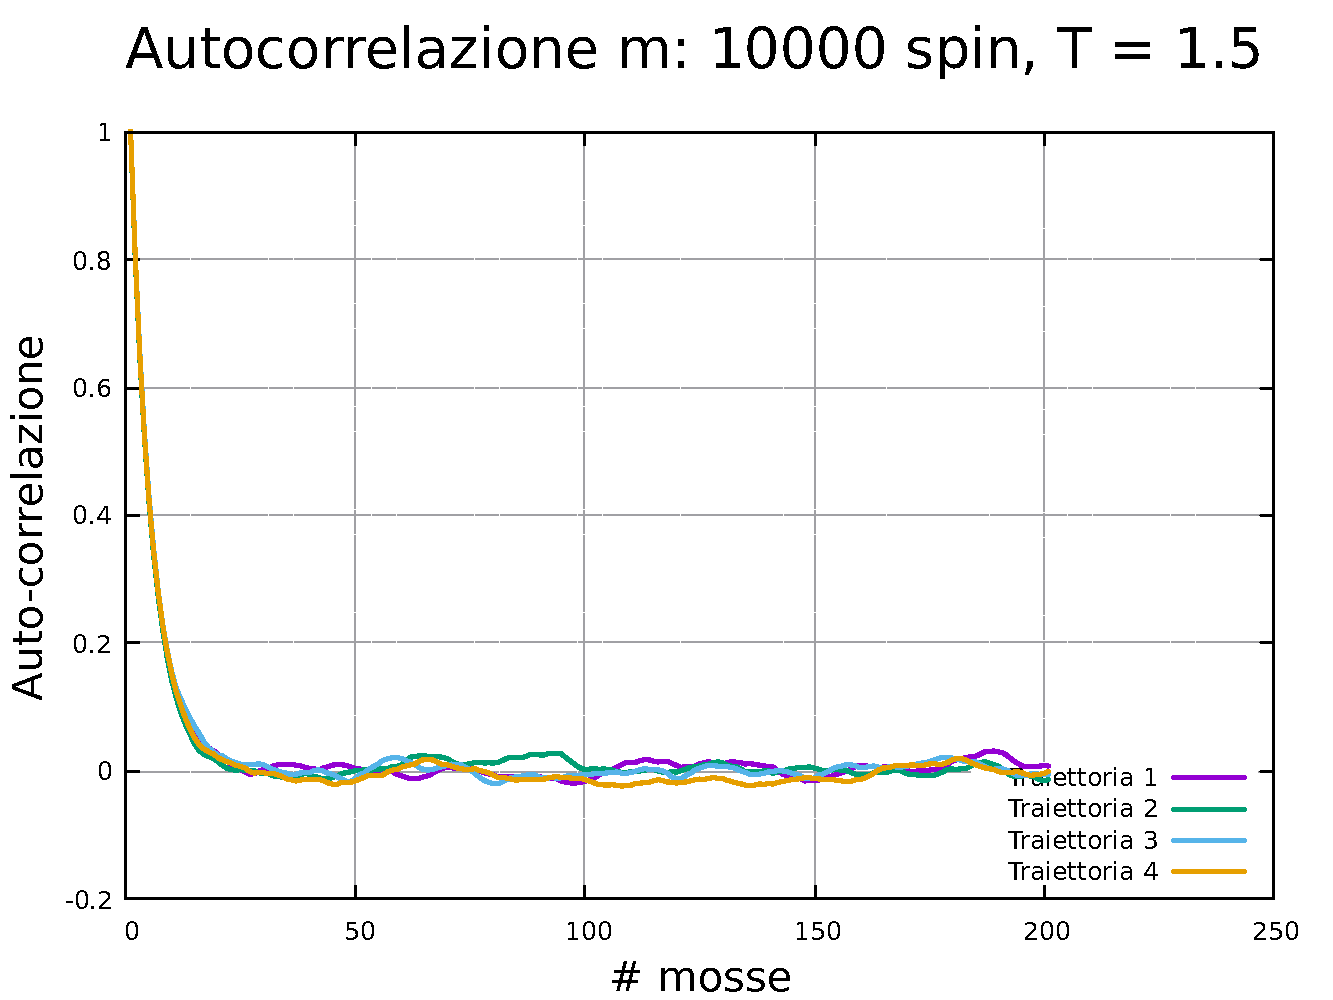
\includegraphics[page=1, width=\textwidth]{Immagini/simIsing1D/magn0.02/tcorr/tcorr_10000_1.5.pdf}
      \caption{$T\,=\,1.5$}
    \end{minipage}\hfill
    \begin{minipage}{0.45\textwidth}  
      \centering
      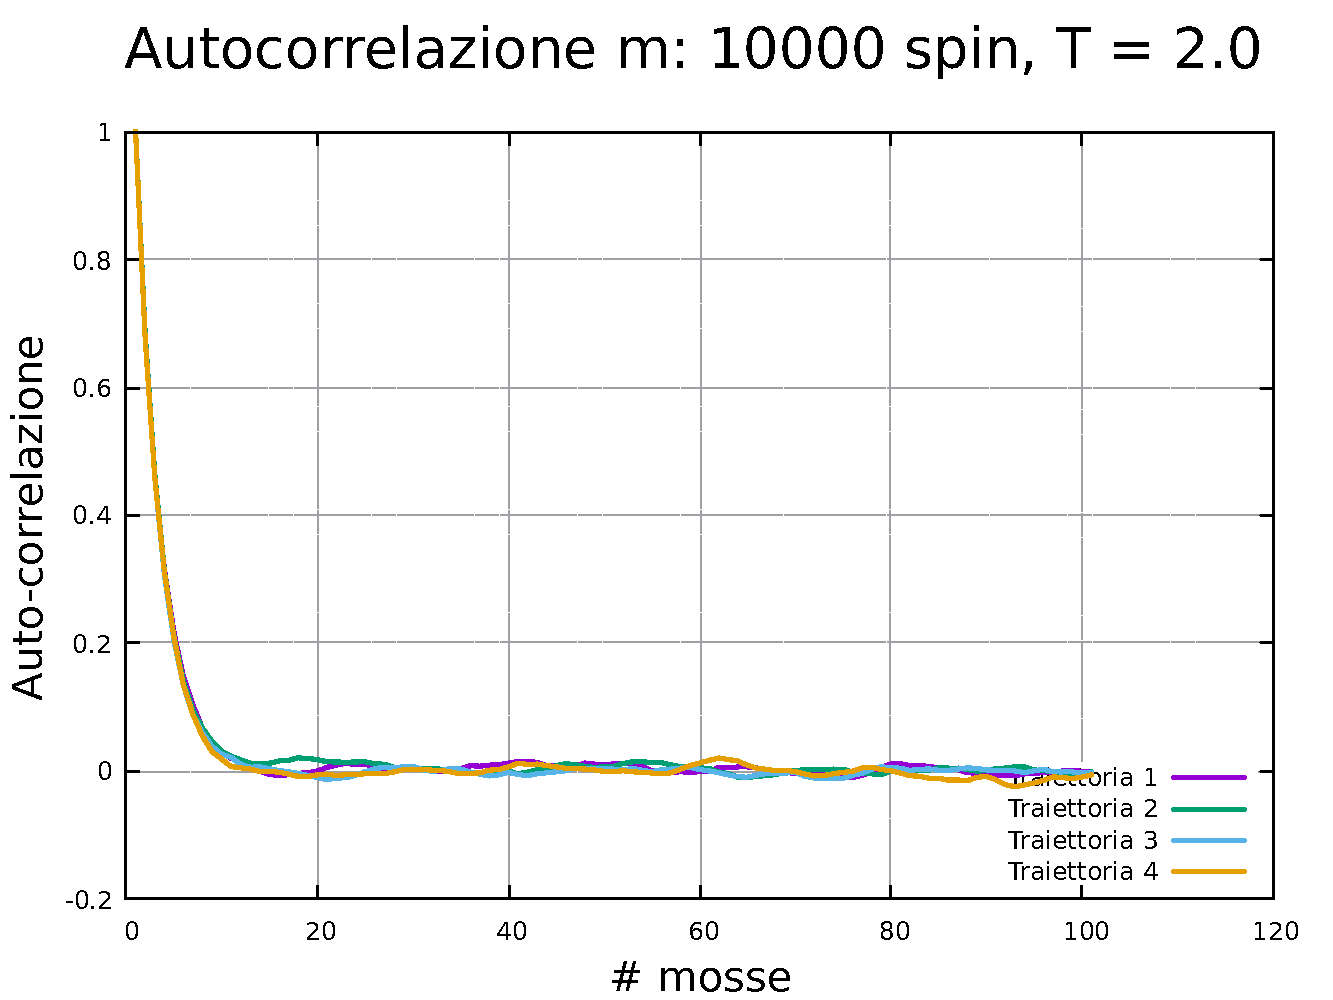
\includegraphics[page=1, width=\textwidth]{Immagini/simIsing1D/magn0.02/tcorr/tcorr_10000_2.0.pdf}
      \caption{$T\,=\,2.0$}
    \end{minipage}
    \caption{Studio dell'auto-correlazione per un modello di Ising 1D costituito da 10000 spin.}
\end{figure}

\vspace*{\fill}

\newpage



\subsubsection{Dimensione dei blocchi}

\vspace*{\fill}

\begin{figure}[htbp]
    \centering
    \begin{minipage}{0.45\textwidth}  
      \centering
      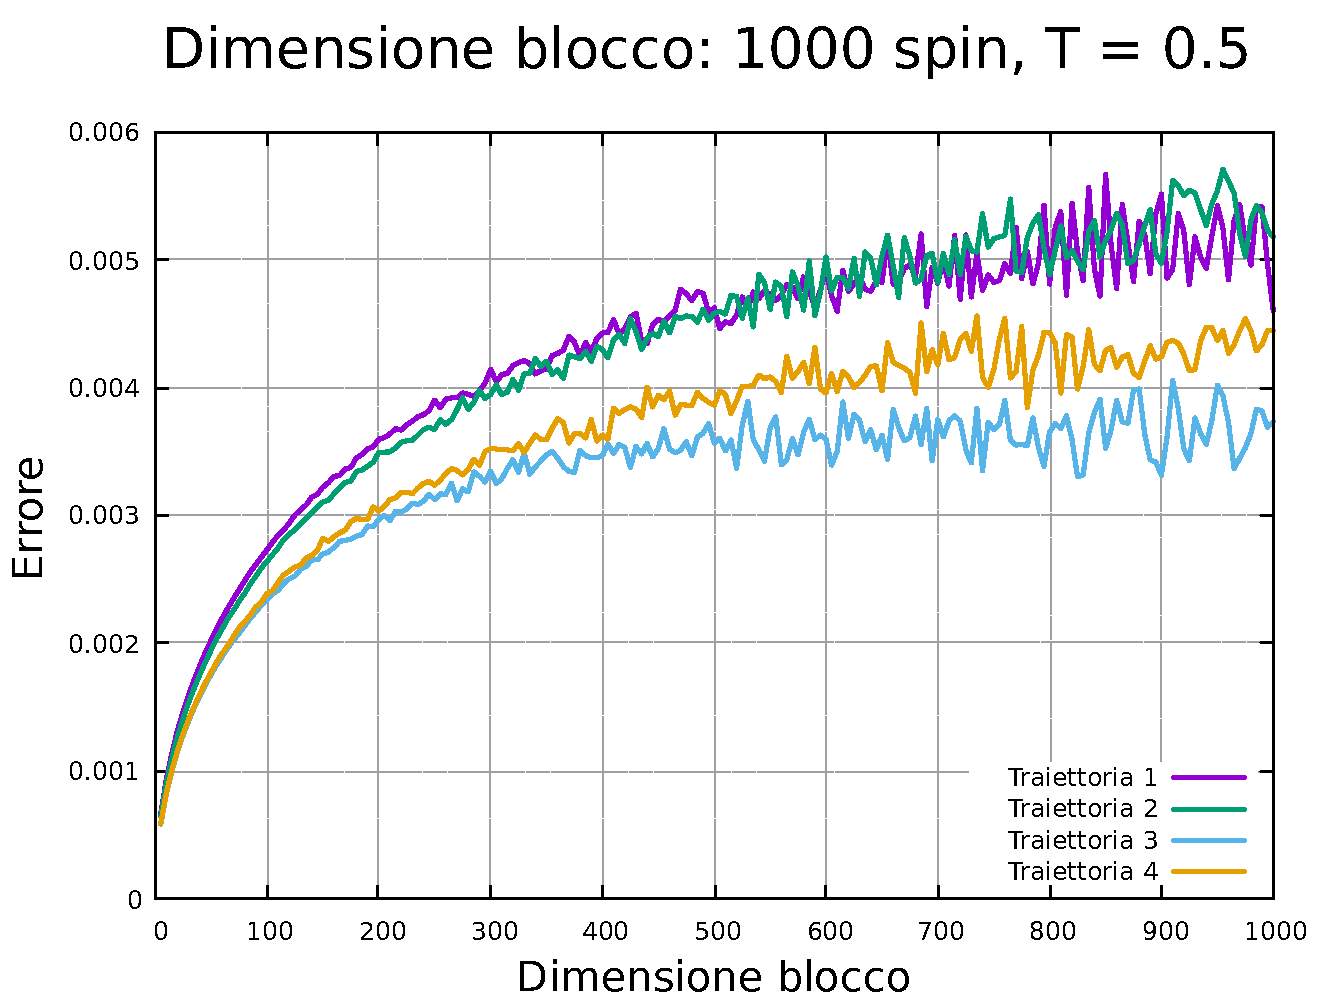
\includegraphics[page=1, width=\textwidth]{Immagini/simIsing1D/magn0.02/lblk/err_1000_0.5.pdf}
      \caption{$T\,=\,0.5$}
    \end{minipage}\hfill
    \begin{minipage}{0.45\textwidth}  
      \centering
      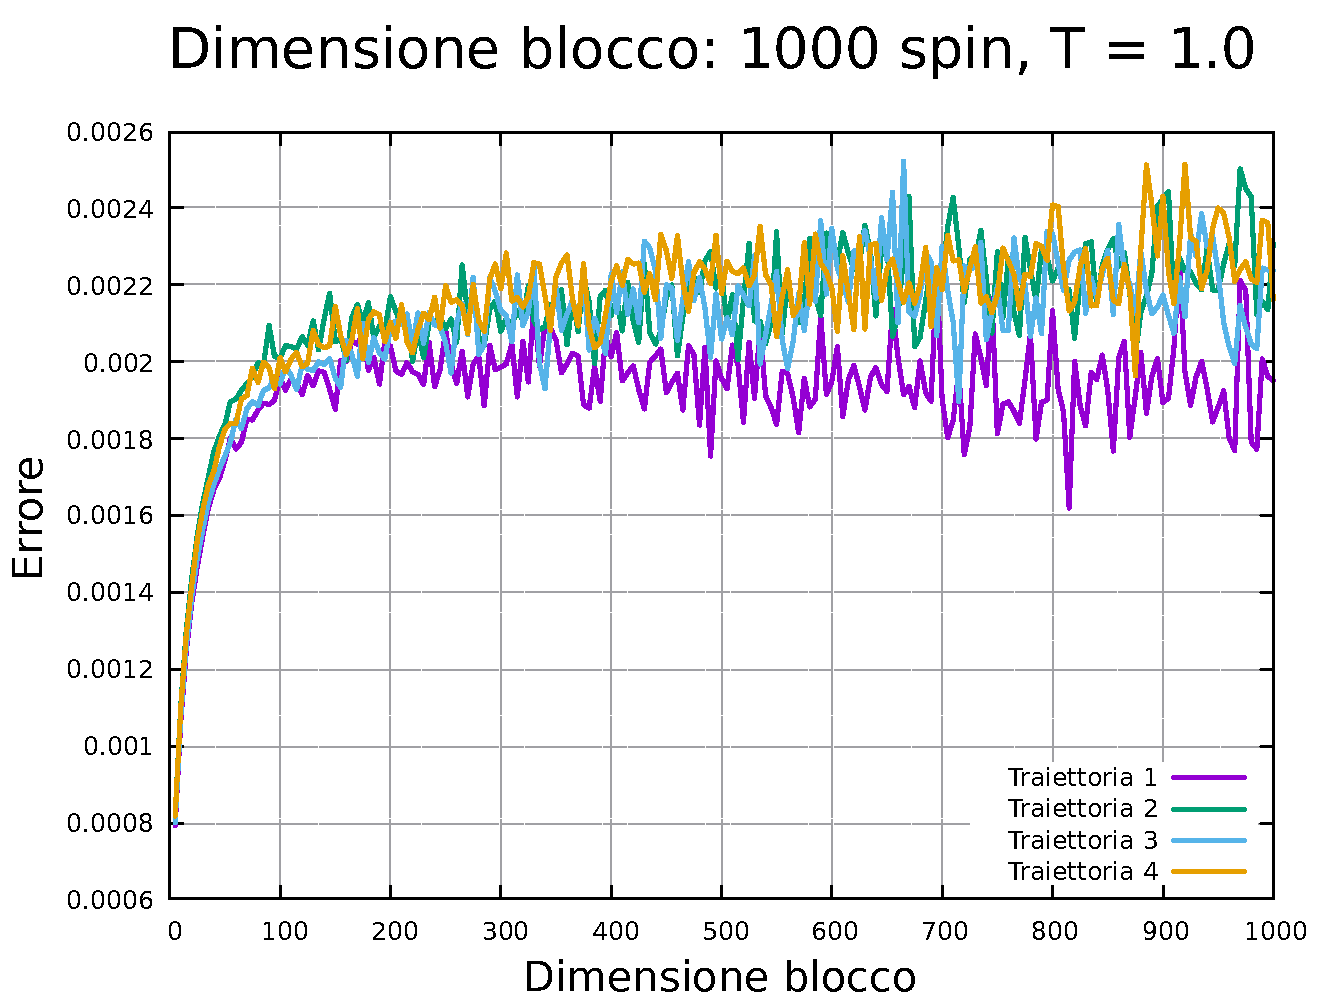
\includegraphics[page=1, width=\textwidth]{Immagini/simIsing1D/magn0.02/lblk/err_1000_1.0.pdf}
      \caption{$T\,=\,1.0$}
    \end{minipage}
    \vskip\baselineskip 
  
    \begin{minipage}{0.45\textwidth}  
      \centering
      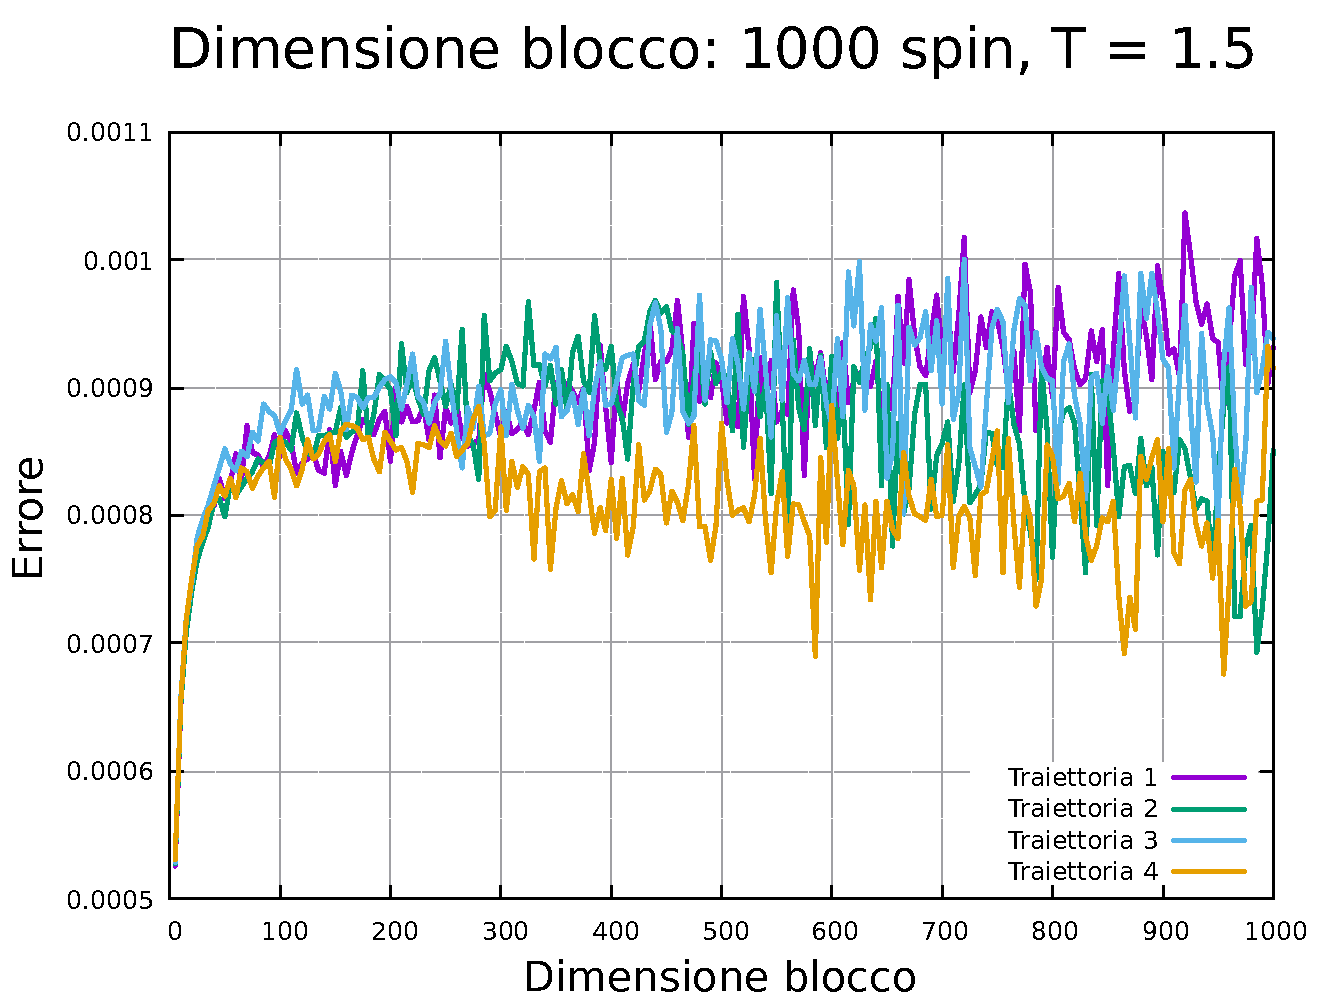
\includegraphics[page=1, width=\textwidth]{Immagini/simIsing1D/magn0.02/lblk/err_1000_1.5.pdf}
      \caption{$T\,=\,1.5$}
    \end{minipage}\hfill
    \begin{minipage}{0.45\textwidth}  
      \centering
      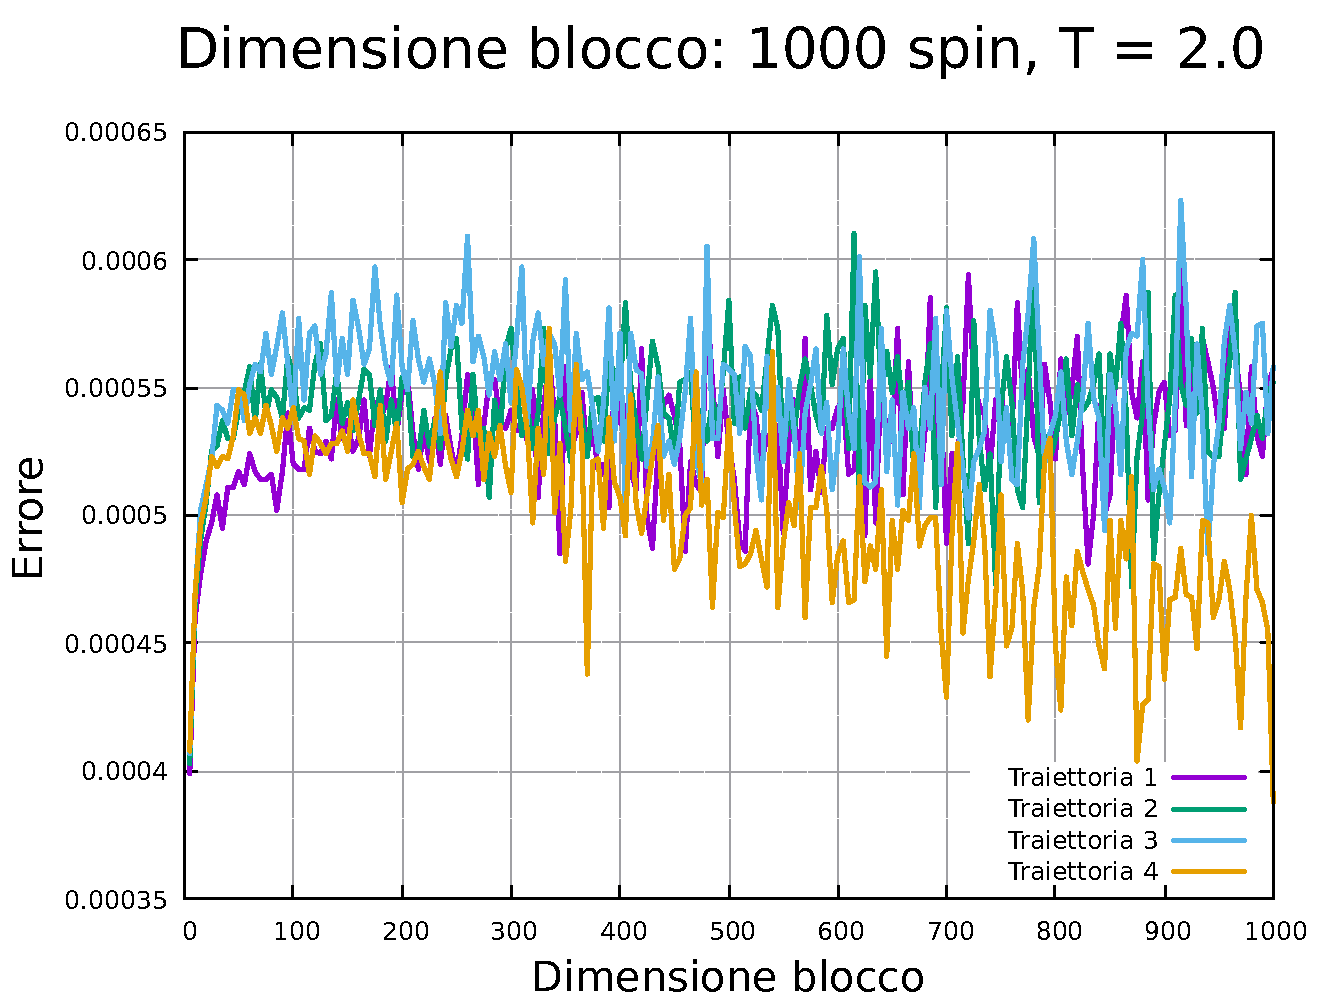
\includegraphics[page=1, width=\textwidth]{Immagini/simIsing1D/magn0.02/lblk/err_1000_2.0.pdf}
      \caption{$T\,=\,2.0$}
    \end{minipage}
    \caption{Errore in funzione della lunghezza dei blocchi per un modello di Ising 1D costituito da 1000 spin.}
\end{figure}

\vspace*{\fill}

\newpage

\vspace*{\fill}

\begin{figure}[htbp]
    \centering
    \begin{minipage}{0.45\textwidth}  
      \centering
      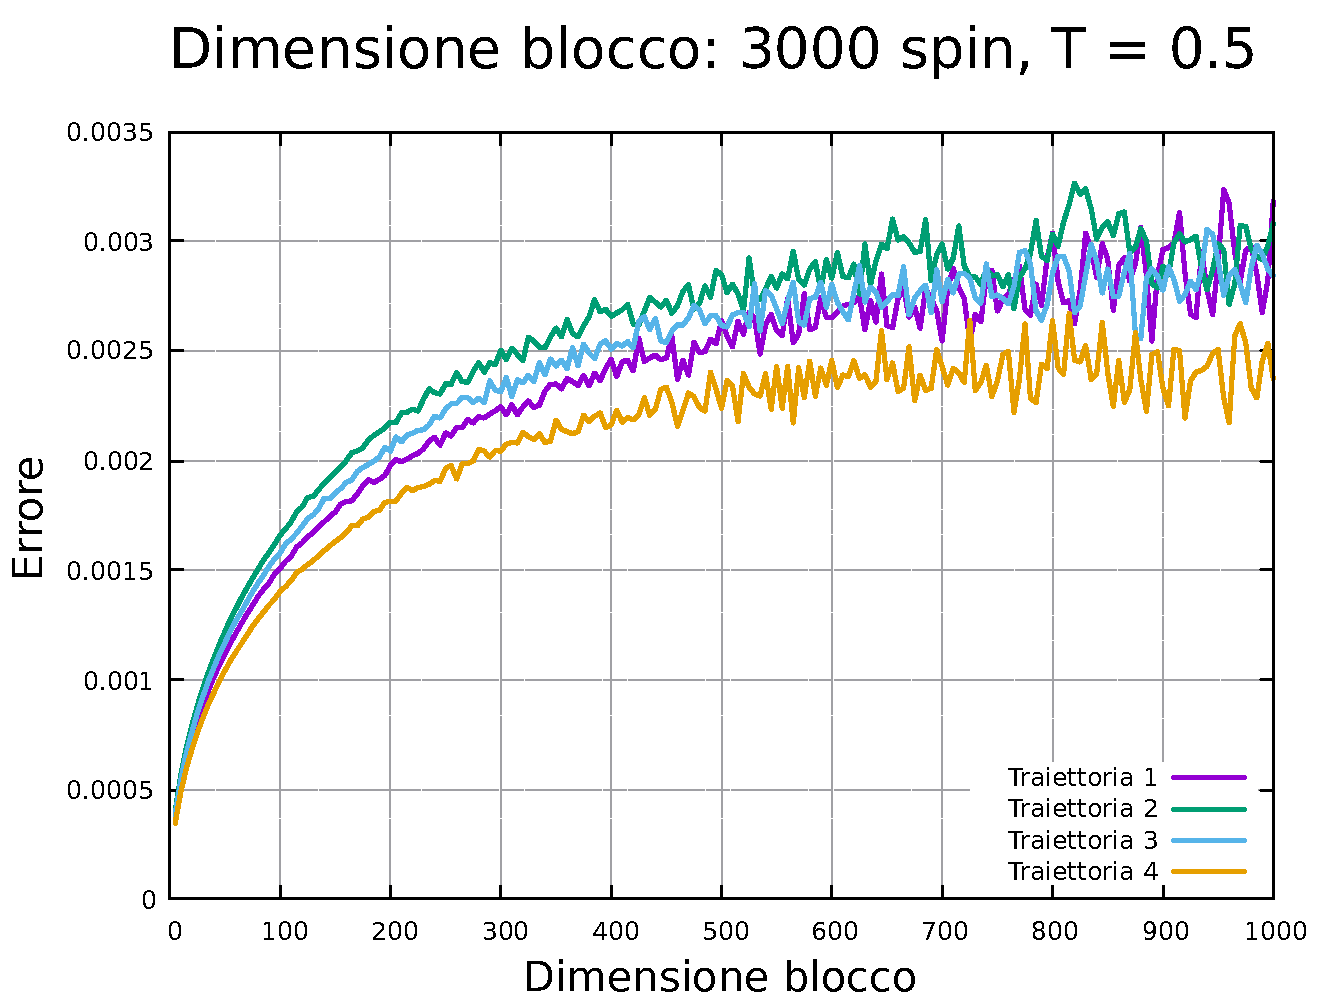
\includegraphics[page=1, width=\textwidth]{Immagini/simIsing1D/magn0.02/lblk/err_3000_0.5.pdf}
      \caption{$T\,=\,0.5$}
    \end{minipage}\hfill
    \begin{minipage}{0.45\textwidth}  
      \centering
      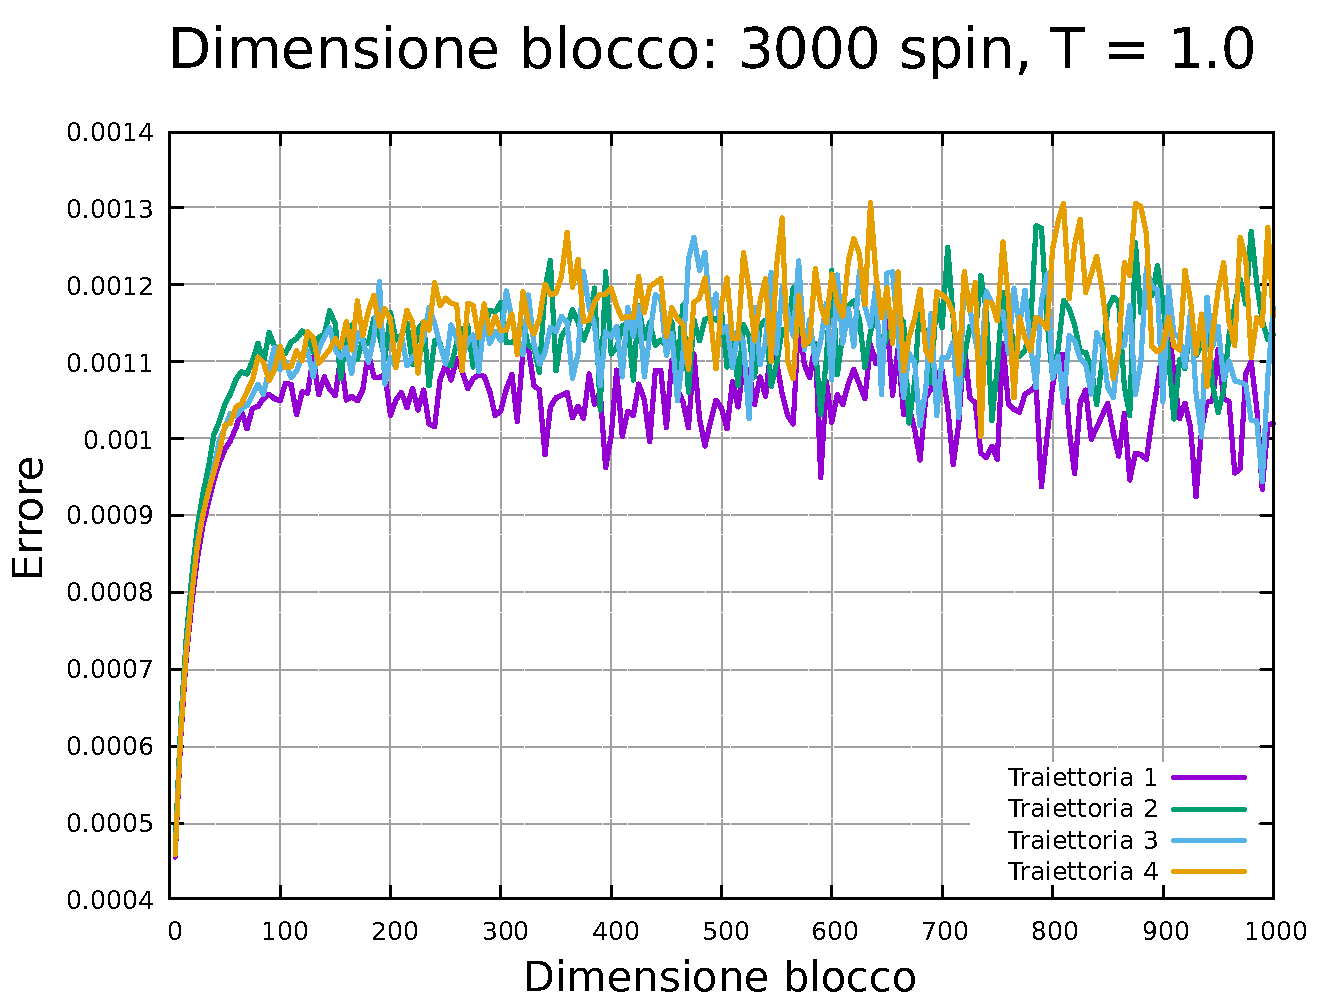
\includegraphics[page=1, width=\textwidth]{Immagini/simIsing1D/magn0.02/lblk/err_3000_1.0.pdf}
      \caption{$T\,=\,1.0$}
    \end{minipage}
    \vskip\baselineskip 
  
    \begin{minipage}{0.45\textwidth}  
      \centering
      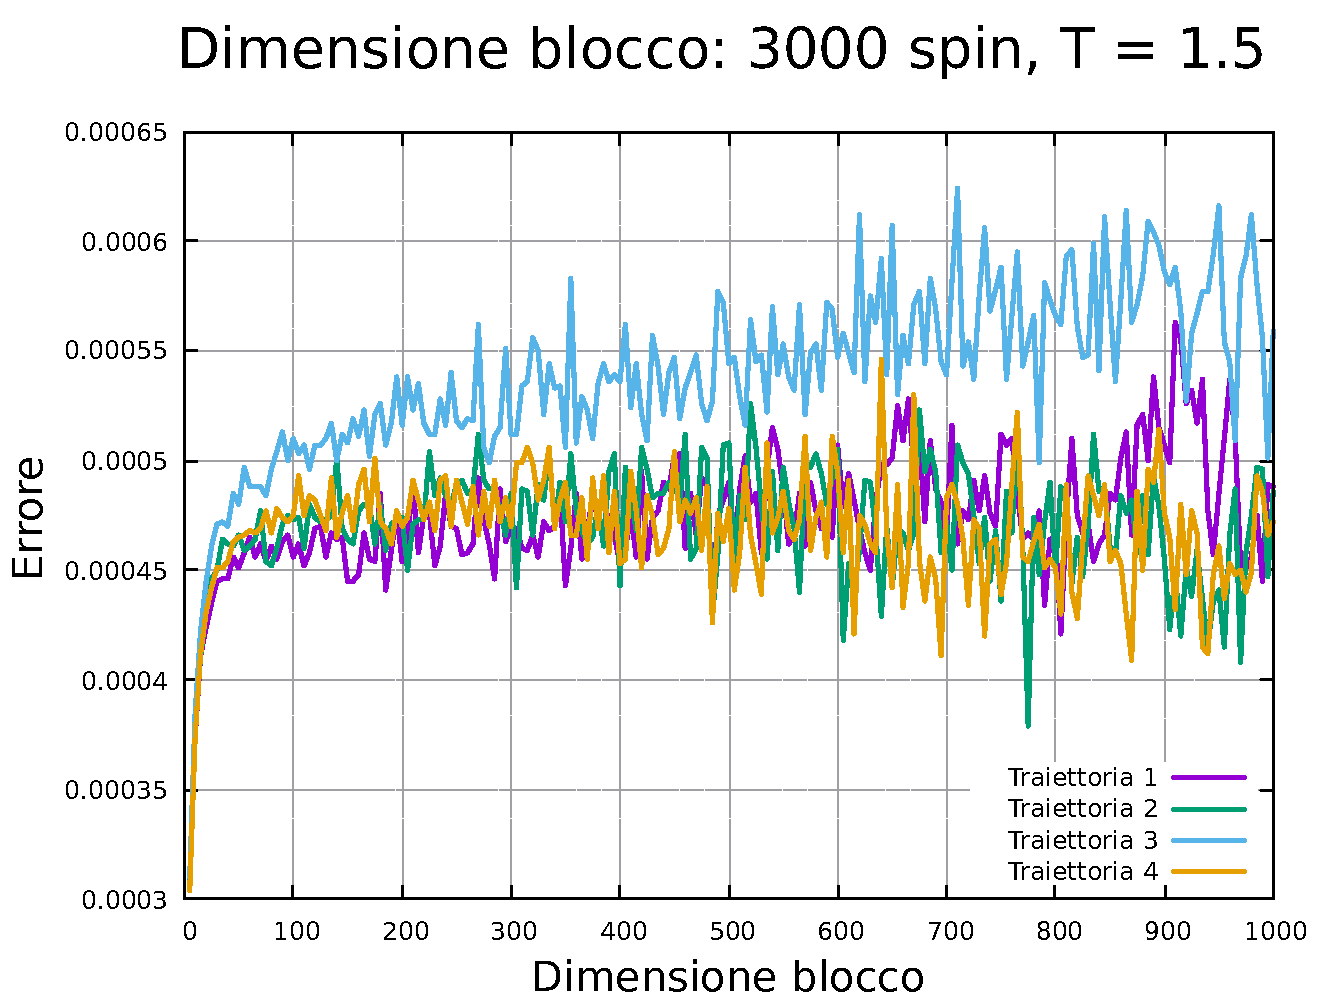
\includegraphics[page=1, width=\textwidth]{Immagini/simIsing1D/magn0.02/lblk/err_3000_1.5.pdf}
      \caption{$T\,=\,1.5$}
    \end{minipage}\hfill
    \begin{minipage}{0.45\textwidth}  
      \centering
      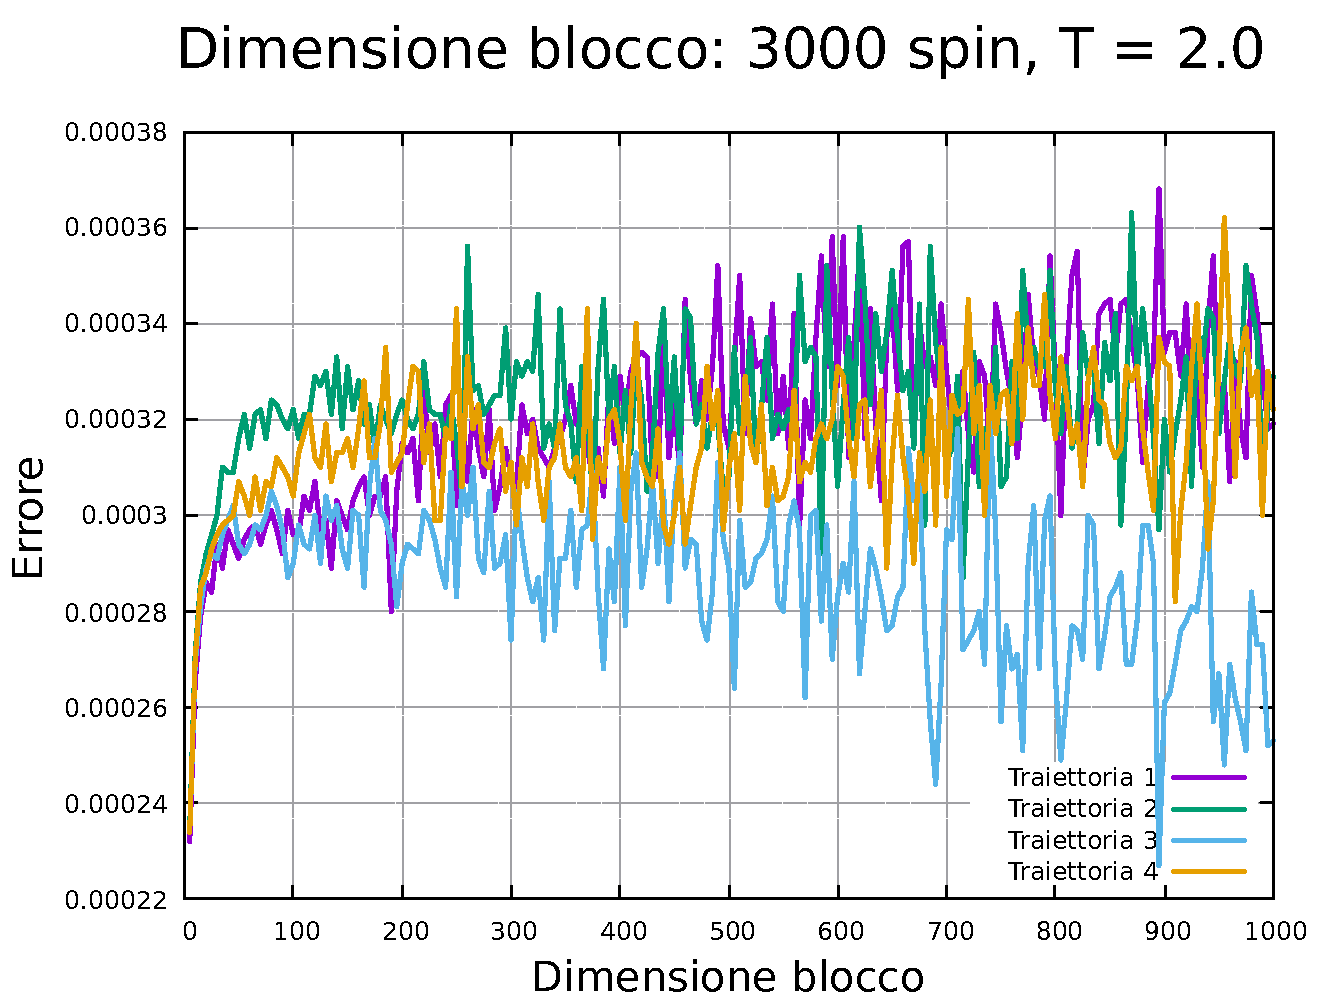
\includegraphics[page=1, width=\textwidth]{Immagini/simIsing1D/magn0.02/lblk/err_3000_2.0.pdf}
      \caption{$T\,=\,2.0$}
    \end{minipage}
    \caption{Errore in funzione della lunghezza dei blocchi per un modello di Ising 1D costituito da 3000 spin.}
\end{figure}

\vspace*{\fill}

\newpage

\vspace*{\fill}

\begin{figure}[htbp]
    \centering
    \begin{minipage}{0.45\textwidth}  
      \centering
      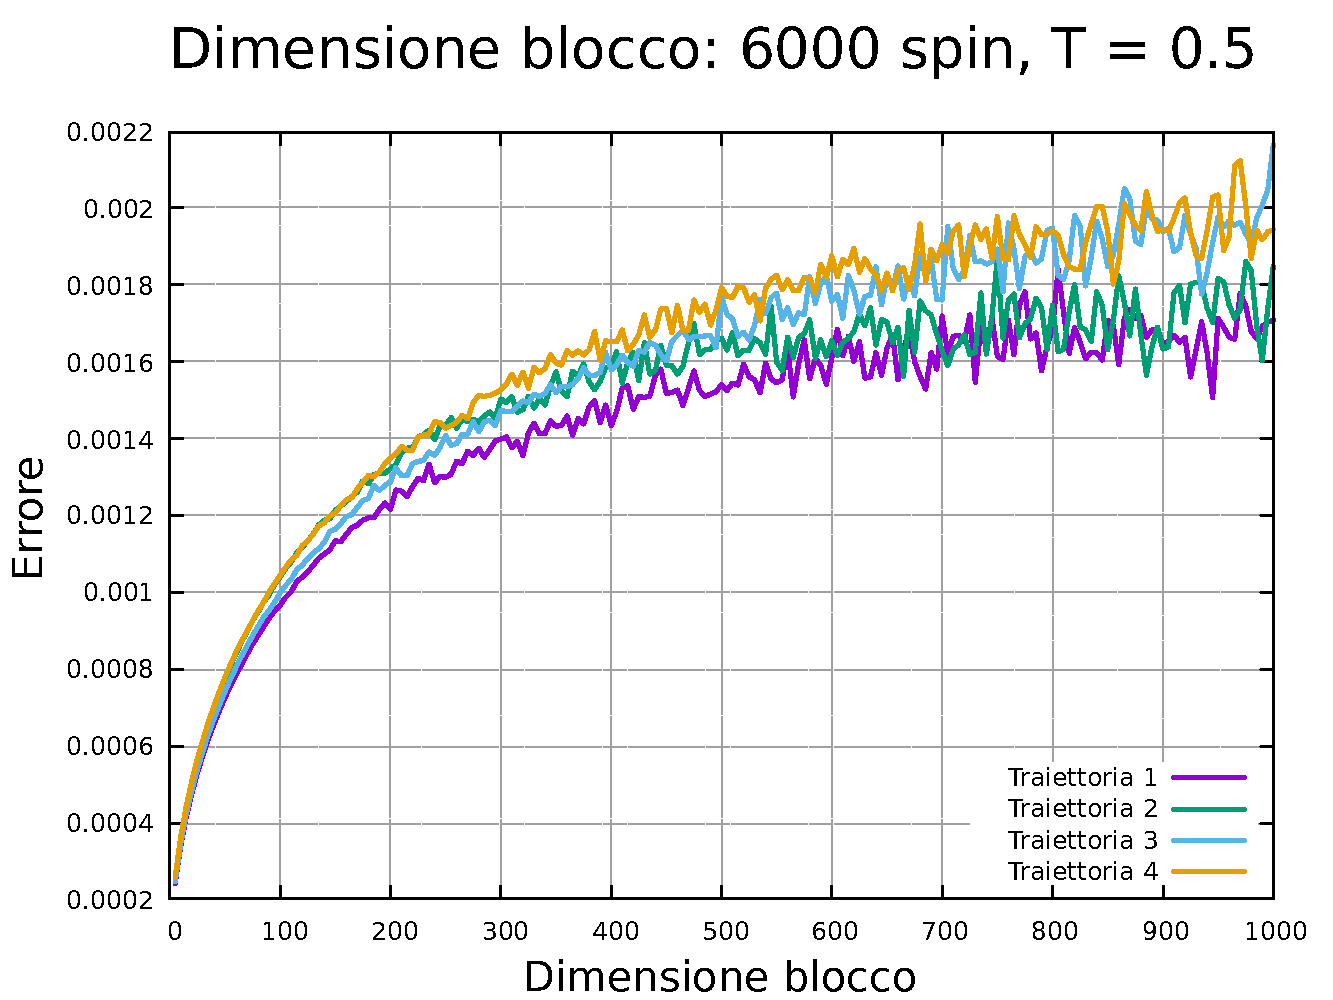
\includegraphics[page=1, width=\textwidth]{Immagini/simIsing1D/magn0.02/lblk/err_6000_0.5.pdf}
      \caption{$T\,=\,0.5$}
    \end{minipage}\hfill
    \begin{minipage}{0.45\textwidth}  
      \centering
      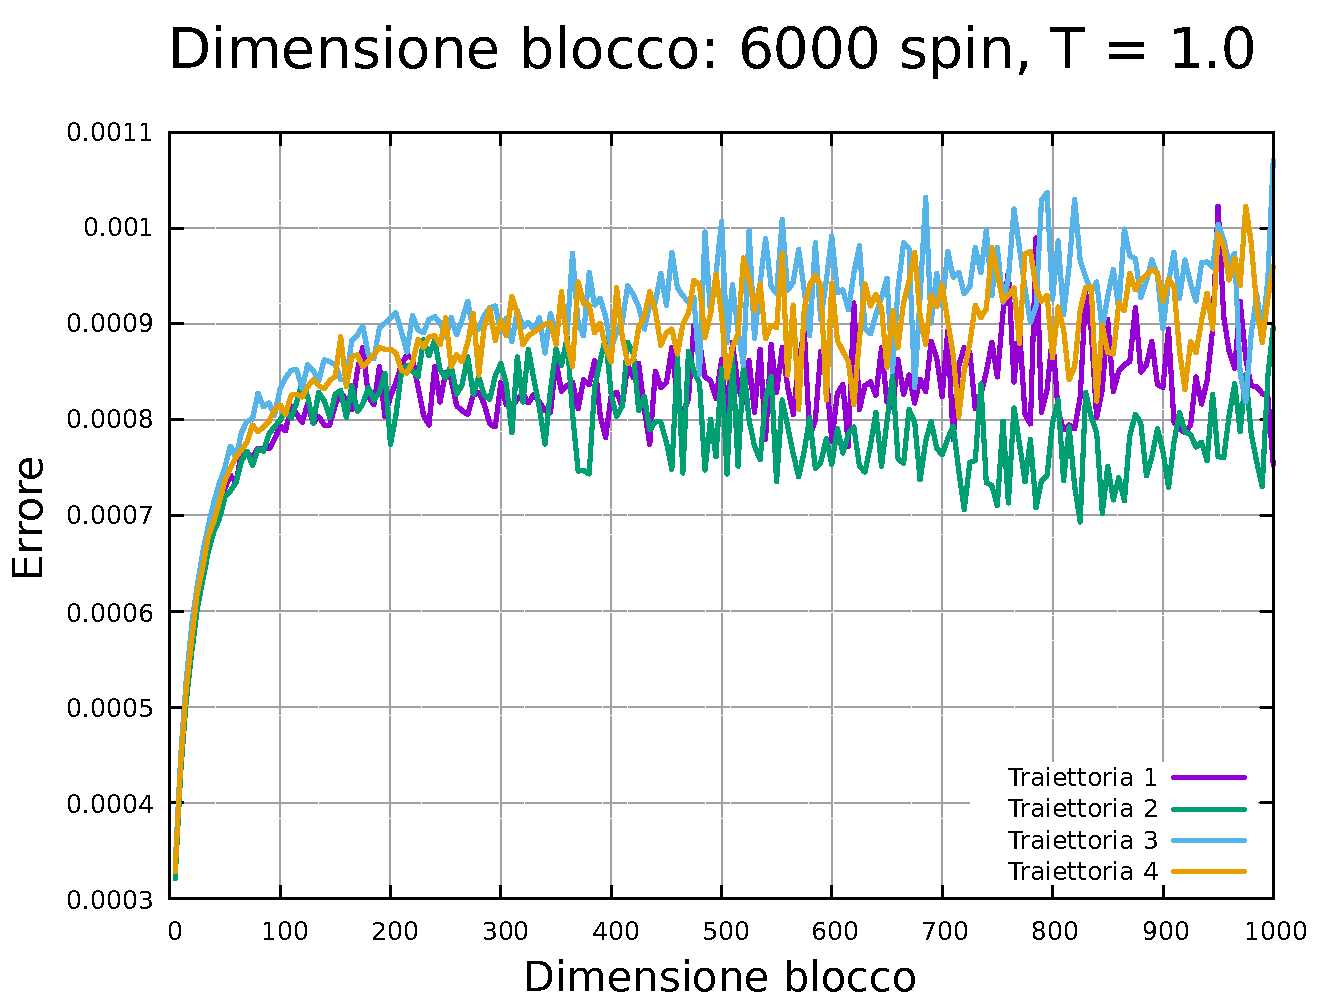
\includegraphics[page=1, width=\textwidth]{Immagini/simIsing1D/magn0.02/lblk/err_6000_1.0.pdf}
      \caption{$T\,=\,1.0$}
    \end{minipage}
    \vskip\baselineskip 
  
    \begin{minipage}{0.45\textwidth}  
      \centering
      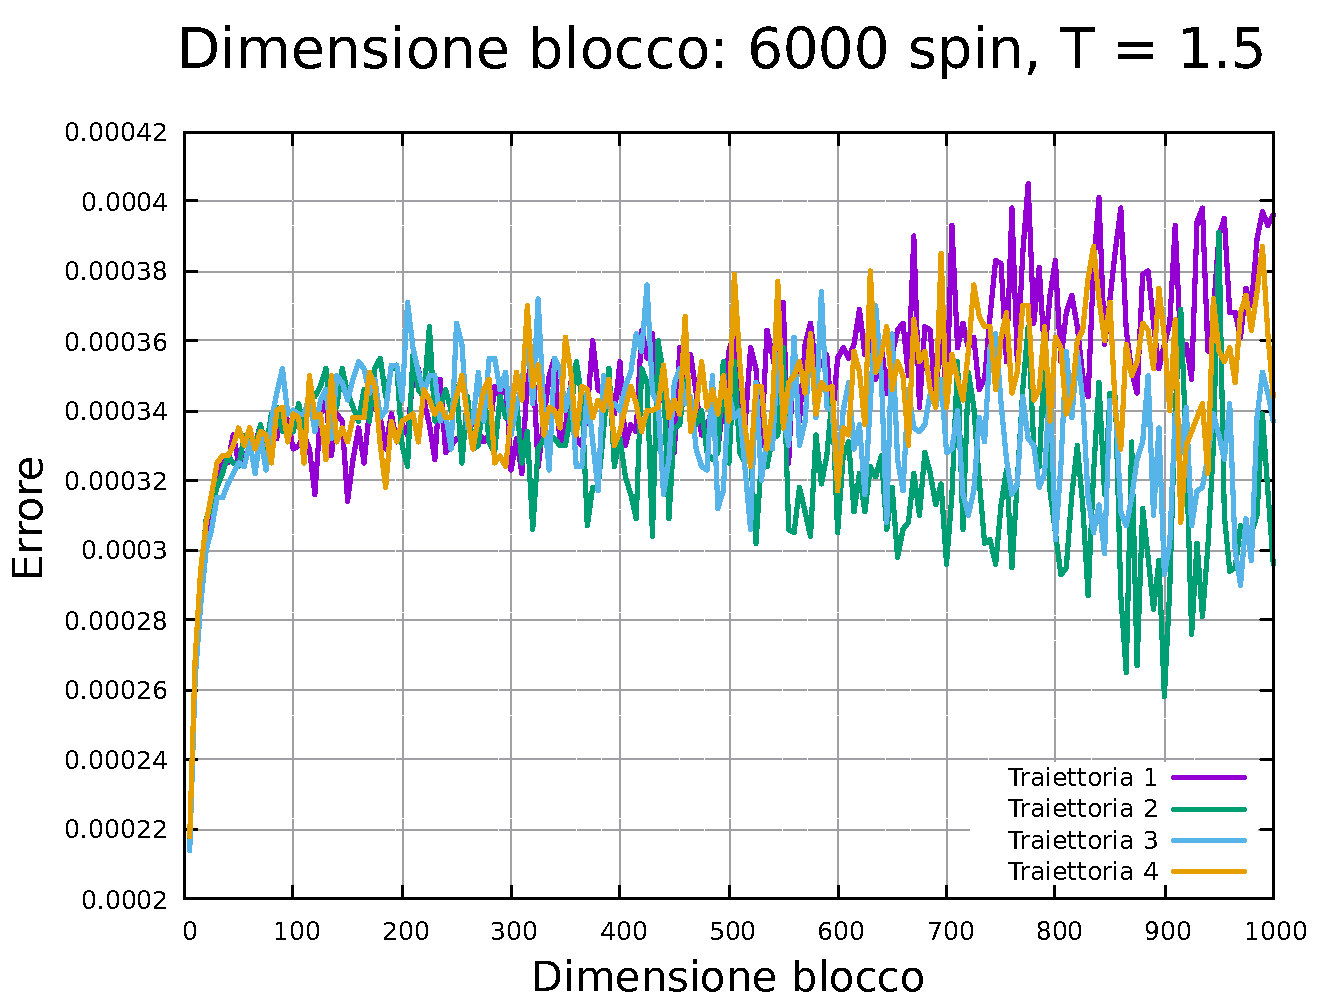
\includegraphics[page=1, width=\textwidth]{Immagini/simIsing1D/magn0.02/lblk/err_6000_1.5.pdf}
      \caption{$T\,=\,1.5$}
    \end{minipage}\hfill
    \begin{minipage}{0.45\textwidth}  
      \centering
      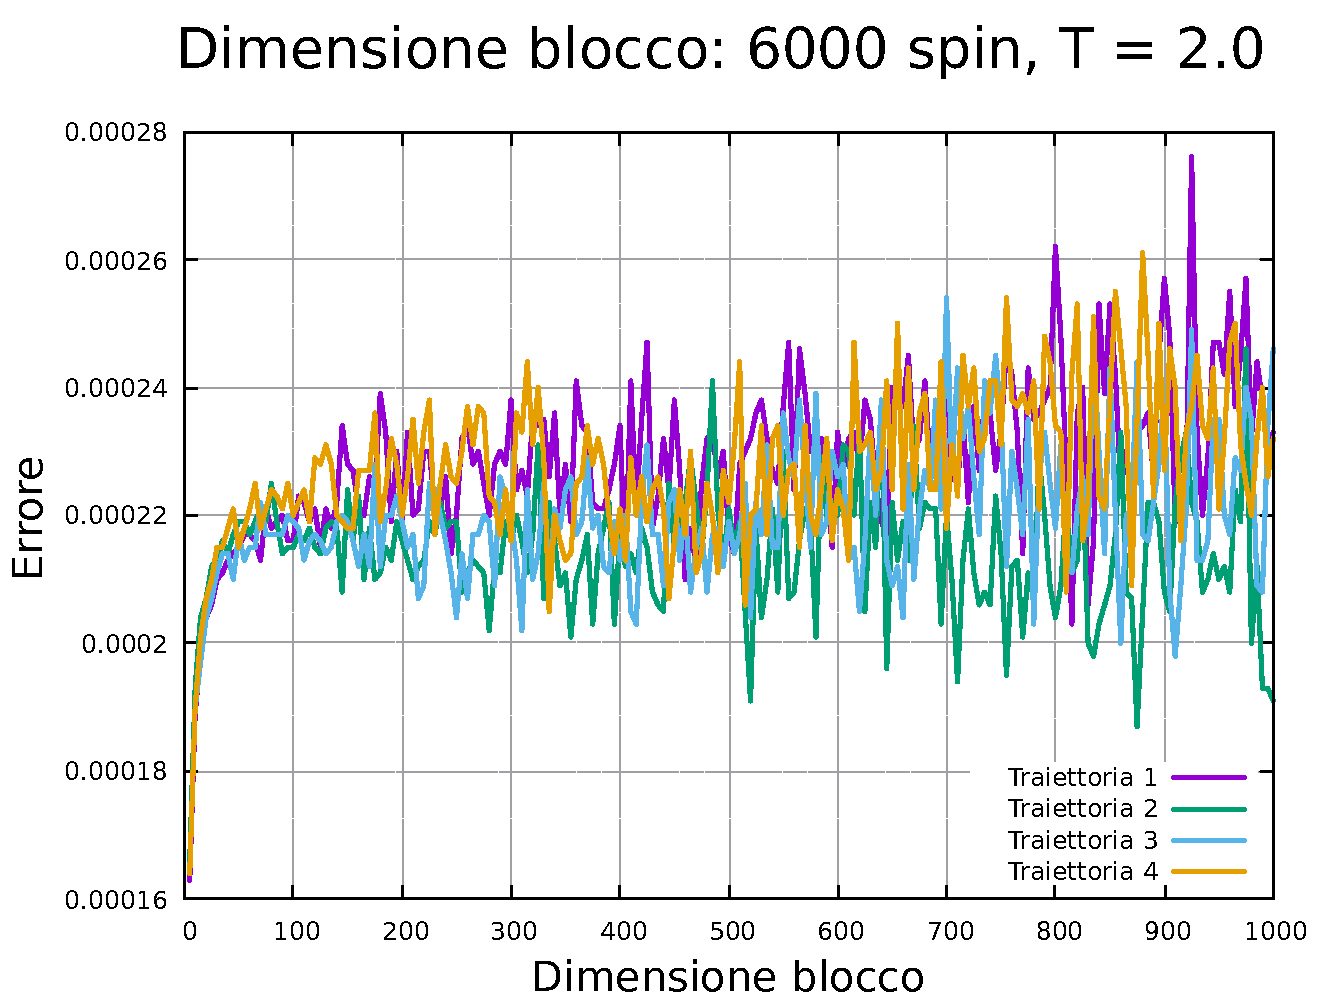
\includegraphics[page=1, width=\textwidth]{Immagini/simIsing1D/magn0.02/lblk/err_6000_2.0.pdf}
      \caption{$T\,=\,2.0$}
    \end{minipage}
    \caption{Errore in funzione della lunghezza dei blocchi per un modello di Ising 1D costituito da 6000 spin.}
\end{figure}

\vspace*{\fill}

\newpage

\vspace*{\fill}

\begin{figure}[htbp]
    \centering
    \begin{minipage}{0.45\textwidth}  
      \centering
      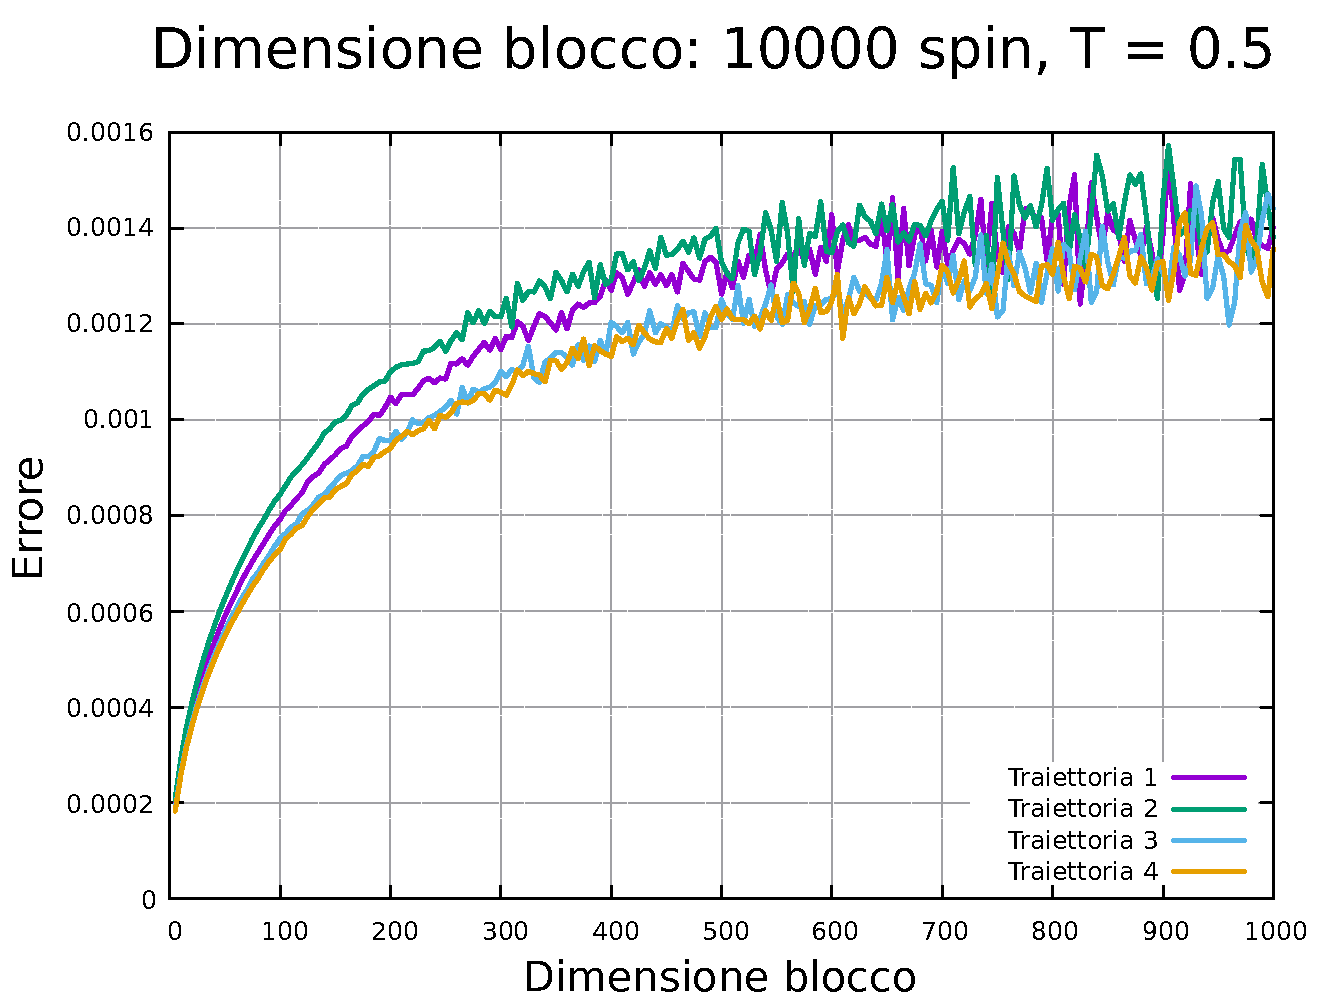
\includegraphics[page=1, width=\textwidth]{Immagini/simIsing1D/magn0.02/lblk/err_10000_0.5.pdf}
      \caption{$T\,=\,0.5$}
    \end{minipage}\hfill
    \begin{minipage}{0.45\textwidth}  
      \centering
      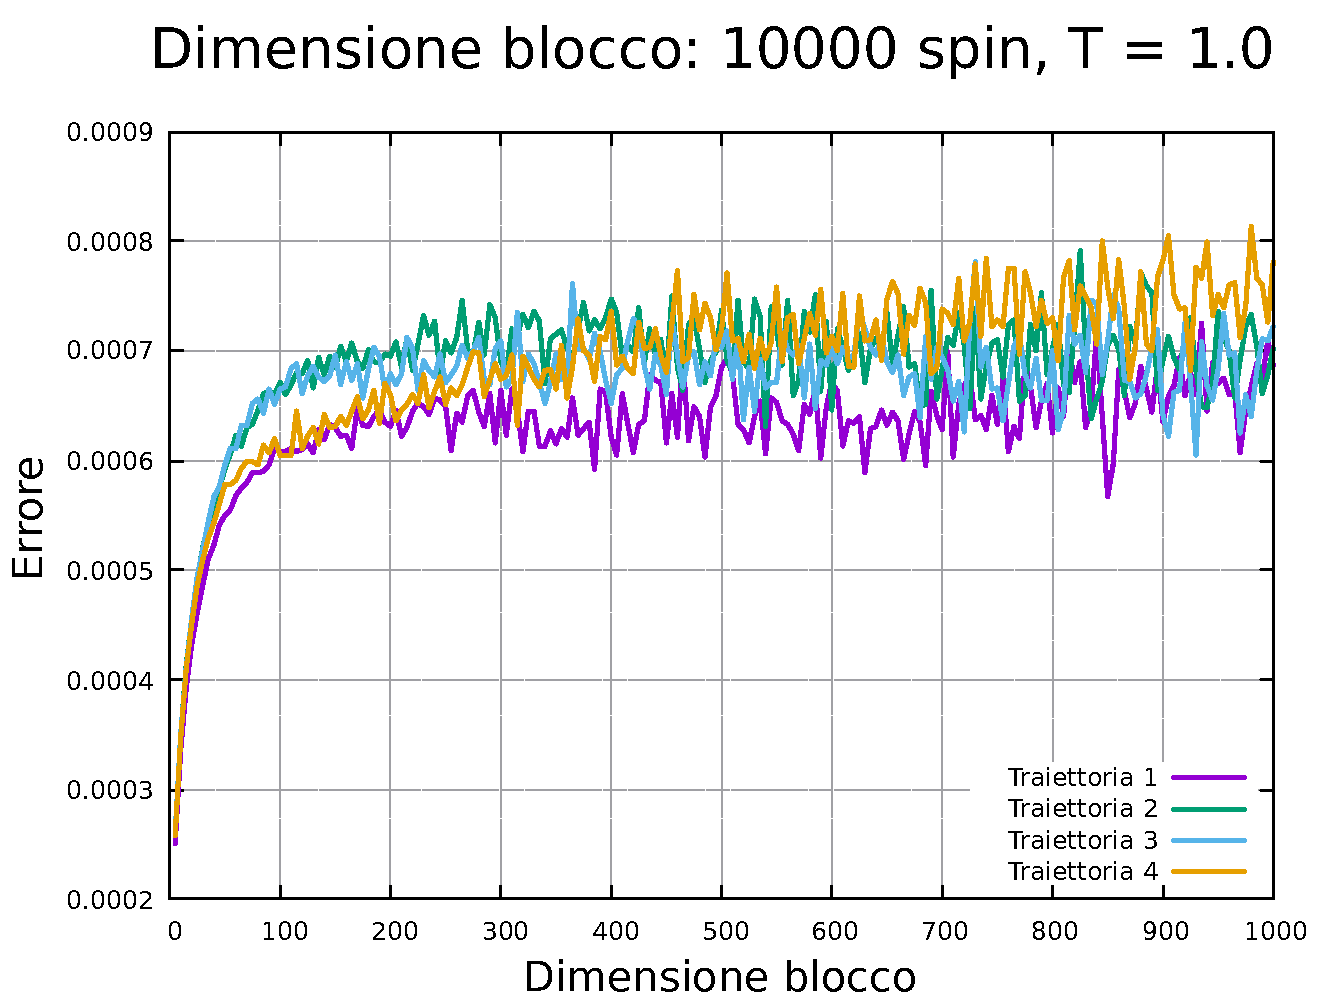
\includegraphics[page=1, width=\textwidth]{Immagini/simIsing1D/magn0.02/lblk/err_10000_1.0.pdf}
      \caption{$T\,=\,1.0$}
    \end{minipage}
    \vskip\baselineskip 
  
    \begin{minipage}{0.45\textwidth}  
      \centering
      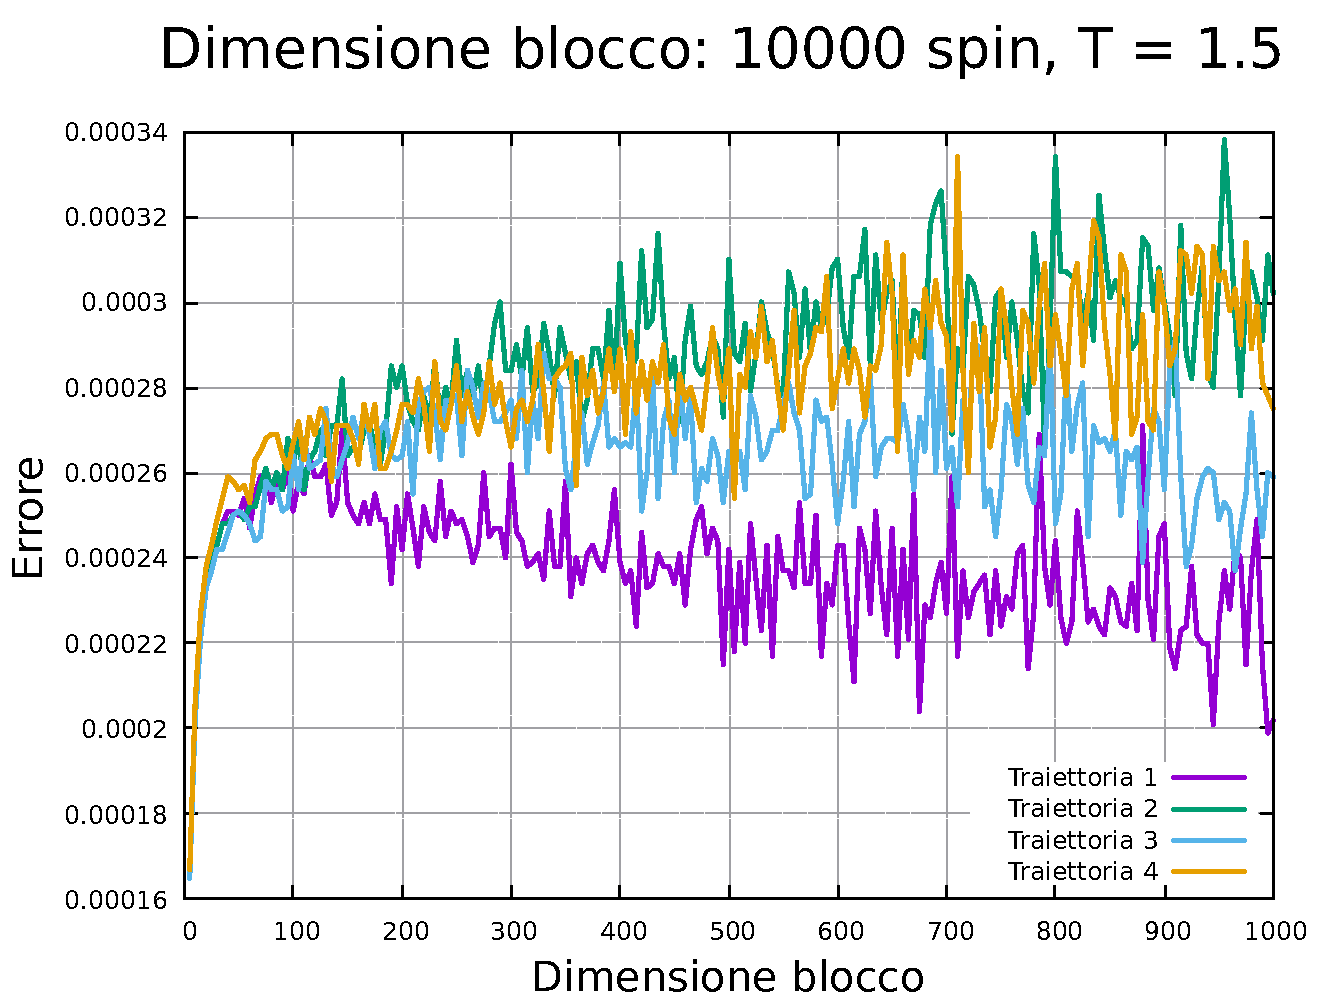
\includegraphics[page=1, width=\textwidth]{Immagini/simIsing1D/magn0.02/lblk/err_10000_1.5.pdf}
      \caption{$T\,=\,1.5$}
    \end{minipage}\hfill
    \begin{minipage}{0.45\textwidth}  
      \centering
      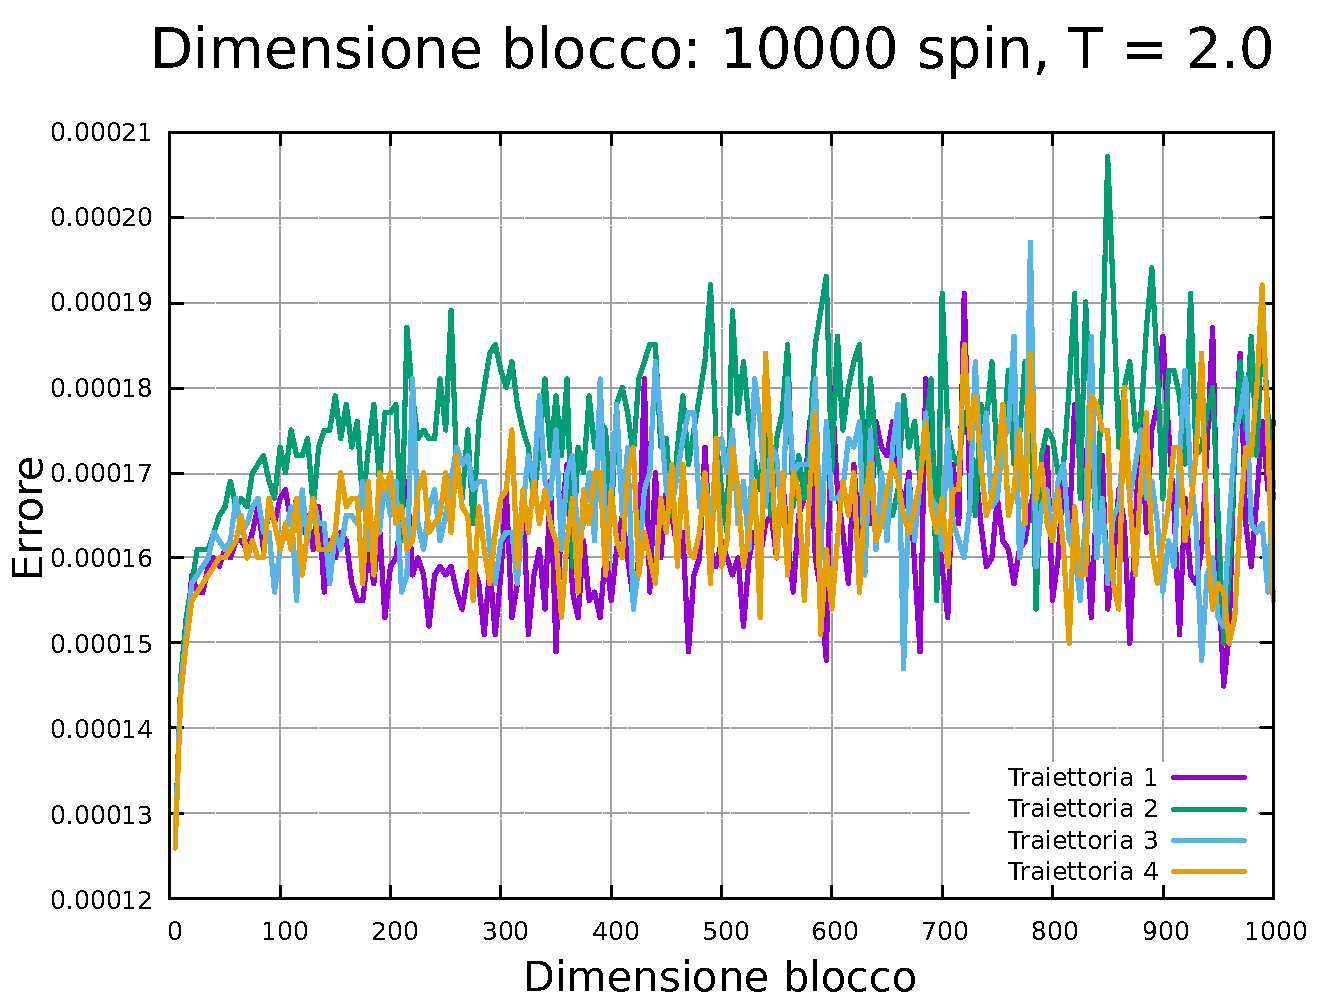
\includegraphics[page=1, width=\textwidth]{Immagini/simIsing1D/magn0.02/lblk/err_10000_2.0.pdf}
      \caption{$T\,=\,2.0$}
    \end{minipage}
    \caption{Errore in funzione della lunghezza dei blocchi per un modello di Ising 1D costituito da 10000 spin.}
\end{figure}

\vspace*{\fill}

\newpage
